\newgeometry{left=3.7cm, right=3.7cm,bottom=4cm ,top=2cm}
\chapter[Neutral MSSM Higgs Bosons Search]{Search for neutral MSSM Higgs Bosons in  
$A/h/H \rightarrow \tau^{+}\tau^{-} \rightarrow e \mu + 4\nu$ decays} \label{chap:anal}


%
 \vspace{0.5cm}

%A search for neutral MSSM Higgs bosons with the ATLAS detector at the
%LHC is presented.  This analysis is based on an integrated luminosity of $20.3 ~fb^{-1}$
%of proton-proton collisions at a centre-of-mass energy of 8 TeV. 
%
%The analysis focusses on the decay of neutral Higgs bosons into a pair of tau
%leptons, which subsequently decay to an electron, a muon and four
%neutrinos. Furthermore, 
%
In the light of the recent discovery of a Higgs 
boson with mass of $\sim 126$ GeV at the LHC~\cite{AHiggsO,CHiggsO}, it remains an open question
whether this new particle is the only missing piece of the electroweak symmetry breaking
sector of the Standard Model or whether it is one of several Higgs bosons predicted in  theories 
that go beyond the SM. The most recent measurements \cite{ASpin0,ACouplings,CFermions,CWidth} of 
properties of the new boson show that they are fully compatible with the ones of the SM Higgs boson. 
Nevertheless, such a new particle can still be accommodated within theories beyond the 
standard model (BSM). Among  them, supersymmetric extensions of the Standard Model are theoretically favoured,
in particular the minimal supersymmetric extesion (MSSM) which predicts five Higgs bosons, three of them electrically neutral.

In this chapter  the search  with the ATLAS detector for the neutral MSSM Higgs bosons decaying into pairs of tau leptons
in the fully leptonic final state is discussed. 
The result have been published in Ref.~\cite{yuppy} as a part of the ATLAS search for the neutral
MSSM Higgs bosons in all final states of the tau lepton decays. 
The search is based on 20.3 $\text{fb}^{-1}$ of  data at a centre-of-mass energy of $\sqrt{s} = 8$~TeV
recorded by the ATLAS experiment during 2012.
This chapter is organised as follows: a brief summary of the MSSM Higgs sector 
and an introduction to the analysis strategy are given in Section~\ref{sec:intro},
while the event selection and categorization are described in Section~\ref{sec:selection}. 
Section~\ref{sec:BackgroundEstimation} describes the estimation of the backgrounds and
in Section~\ref{sec:Systematics} methods for the evaluation of the  systematic uncertainties are discussed. Finally, 
in Section~\ref{sec:result} the result of the search are presented togheter with an overview of the statistical methods employed.


%There are two approach to explore the Higgs sector:
%one can study the coupling of the Higgs boson with vector
%bosons and fermions, those measure in fact are sensitive to new physics and can determine
%%given the unitarily property of scattering
%%amplitudes for longitudinal vectors and fermions, one can understand 
%if this particle is  fully responsible for
%the generation of all the SM particles masses. 
%Another approach is to directly search for %model dependent
%for additional Higgs es in a well defined model, which is the approach followed in this
%thesis where new neutral bosons are sought within the MSSM (see chapter \ref{}). 
%
%
%%Discovering the mechanism responsible for electroweak
%%symmetry-breaking and the origin of mass for elementary particles has been
%%one of the major goals of the physics program at the Large Hadron
%%Collider~(LHC)~\cite{LHC}.  In the Standard Model (SM) this mechanism
%%requires the existence of a single scalar particle, the Higgs
%%boson~\cite{ENGLERT,HIGGS,HIGGS2,HIGGS3,Guralnik:1964eu}.
%
%%This chapter is divided in three sections:
%%in section~\ref{sec:strategy} an introduction to experimental searches and to the strategy
%of this particular analysis is given, in section~\ref{sec:bkg} is described the core of this thesis
%work, i.e. the detail of the background modelling for this analysis, while in section~\ref{sec:result}
%the result of the search are presented.


\restoregeometry
\clearpage
\newpage

\section{Introduction } \label{sec:intro}

\subsection{The Higgs Sector in the MSSM}

\begin{figure}[tp]
     \begin{center}

            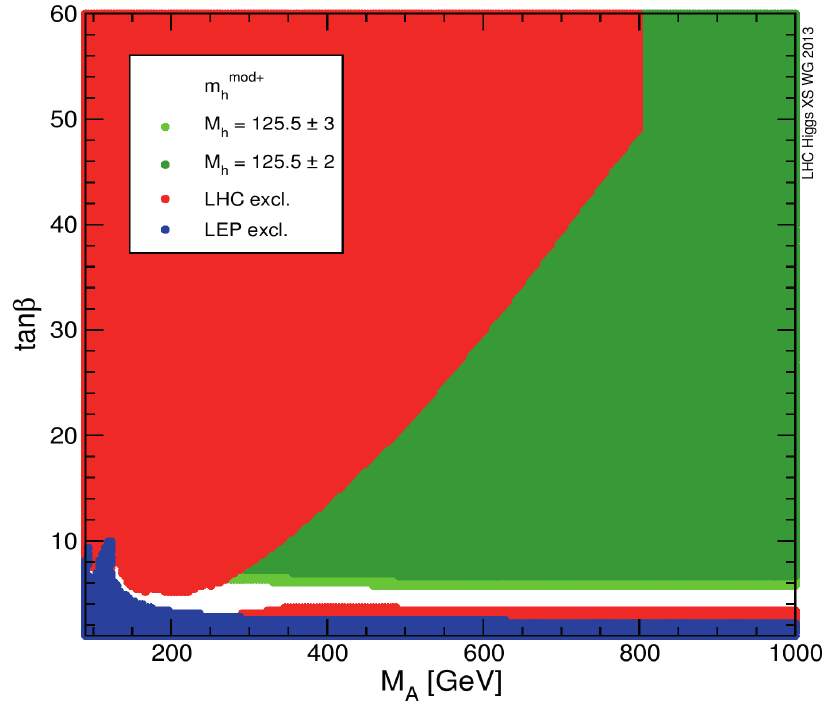
\includegraphics[width=0.7\textwidth]{figure/mh_mod.png}

    \end{center}
    \caption{Excluded and allowed regions of the MSSM  $m_{A} - \text{tan}\beta$ parameter space in the $m_{h}^{mod+}$ 
	benchmark scenario~\cite{LHCxsec}, based on direct Higgs boson searches at LEP 
	(blue) and LHC (red). The two green regions are compatible with the assumption that 
	the lightest MSSM Higgs boson, \emph{h}, has a mass of 125.5~GeV with an uncertainty of 2~GeV (dark green) 
	or 3~GeV (light green). }
   \label{fig:mhmod}
\end{figure}

In the minimal supersymmetric extension of the Standard Model
(MSSM)~\cite{MSSM1, MSSM2}, the Higgs sector is composed of two electroweak Higgs
doublets of opposite hyper-charge resulting in five observable Higgs
bosons, where two of them are neutral and $CP$-even
($h$,$H$), one is neutral and $CP$-odd ($A$) and two are charged
($H^\pm$).  At tree level, their properties such as masses, widths and
branching ratios are predicted depending on  only two parameters,
often chosen to be the mass of the $CP$-odd Higgs boson $m_A$ and
the ratio of the vacuum expectation values of the two Higgs doublets
$\tan\beta$ (for more details see chapter~\ref{chap:theory}).  
The MSSM predicts the existence of a Higgs boson with properties that  
resemble those of the SM Higgs boson in large regions of its parameter space. 
This is usually the case for the lightest Higgs boson, \emph{h}, while the other two, $H$ and $A$, 
tend to be degenerate in mass and decouple from gauge bosons.
%Production and decay mode 
%with vector bosons are forbidden for the CP-odd, $A$ and are suppressed for 
%the CP-even, $H$, Higgs bosons. 
On the other hand, the couplings of the latter two Higgs bosons to down (up) type fermions are enhanced
(suppressed) depending on the value of $\tan\beta$, such that for large $\tan\beta$
bottom-quarks and $\tau$ leptons  play an important role for Higgs boson production and decay. 
 
The two dominant neutral MSSM Higgs boson production mechanisms 
at the LHC are gluon fusion, $gg\rightarrow A/H/h$, and 
the production in association with $b$-quarks, $pp \rightarrow b(b)A/h/H$, the latter becoming increasingly 
important for large values of $\tan\beta$. These  are the only production mechanisms
considered in this analysis. 
Assuming there are no decays into supersymmetric particles  (since they are too heavy)
and assuming that the lightest neutral CP-even Higgs boson $h$ is identified with the observed Higgs boson
of mass $\sim 126$~GeV, the dominant decay mode for the neutral MSSM CP-odd $A$ and CP-even $H$ Higgs bosons
 is the decay into a  $b$ and anti-$b$ quark pair, % $A/h/H \rightarrow b\bar{b}$, 
followed by the decay into $\tau$ leptons pairs. Since it is very difficult to distinguish the former decay 
from the large $b\bar{b}$ background, the decay mode 
$A/h/H \rightarrow \tau^+ \tau^-$  provides the highest sensitivity in the search for neutral MSSM Higgs bosons.

Searches for neutral MSSM Higgs bosons have been performed at
LEP~\cite{LEPLimits}, the
Tevatron~\cite{TevatronLimits1} and the LHC~\cite{CMSLimit, ATLASLimit}. 
In the following, the search for the neutral MSSM Higgs bosons  in the final state 
$A/h/H \rightarrow \tau^+ \tau^- \rightarrow e \mu +4\nu$ is presented. 
This search is complementary to the searches in other $\tau^+\tau^-$ final states
characterised by the presence of one or two hadronicaly decaying $\tau$ leptons. For low $m_A$ values
the $\tau^+ \tau^- \rightarrow e \mu +4\nu$ search channel provides a sensitivity to the signal comparable to the 
other final states, despite  the fact that the $\tau\tau$ branching ratio to $e \mu +4\nu$ is only 6\%. 
This is mainly due to the high transverse momentum threshold at the trigger level for  hadronicaly decaying $\tau$ leptons,
which is necessary to keep the jet contamination rate at an acceptable level.

As it is virtually impossible to explore the full parameter space of the MSSM, 
which has a large number of free parameters, several benchmark scenarios have been  
introduced  fixing all paramenters except $m_A$ and $\tan\beta$  to typical values for the most interesting 
physics cases.
With the recent Higgs boson discovery, benchmark scenarios of the MSSM have been updated to 
accommodate the  new experimental constraints. 
As an example, Figure~\ref{fig:mhmod} shows the currently excluded and allowed regions of the MSSM $m_{A} - \text{tan}\beta$ 
parameter space for the updated  $m_{h}^{mod+}$ benchmark scenario (see Section~\ref{sec:benchmark}). 
In this scenario, a large region of the $m_{A} - \text{tan}\beta$
parameter space is compatible with the assumption that the observed Higgs boson is in fact the 
neutral CP-even  Higgs boson $h$. A relatively large part of this parameter space is still experimentally unexplored,
which is a strong motivation to pursue the search for additional neutral MSSM Higgs bosons.


\subsection{Signal and Background Processes}
Signal events in which the neutral MSSM Higgs bosons decay through 
$A/h/H \rightarrow \tau^+ \tau^- \rightarrow e \mu +4\nu$  are characterised 
by the presence of one electron and one muon of opposite charge. These two leptons are isolated and have 
relatively high transverse momenta. In addition, four neutrinos generate high missing transverse energy in the event. 
Figure~\ref{fig:feyndiagSignal} shows leading order Feynman diagrams for the two signal production modes considered,
gluon fusion and  associated production  with $b$-quarks.
The presence (absence) of a b-jet in the final state serves as  main characteristic for the categorization
in the latter (former) event as described below.

\begin{figure}[tp]
     \begin{center}
     \subfigure[]{		
            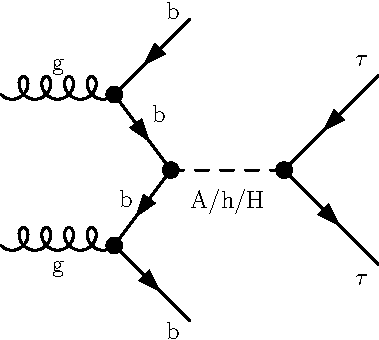
\includegraphics[height=3.5cm]{feyn_diagrams/diagrams/bbA.pdf}
     }\hspace{0.2cm}	
     \subfigure[]{		
            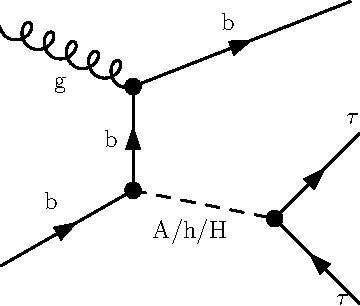
\includegraphics[height=3.5cm]{feyn_diagrams/diagrams/bbA2.pdf}
     }	\hspace{0.2cm}	
     \subfigure[]{		
            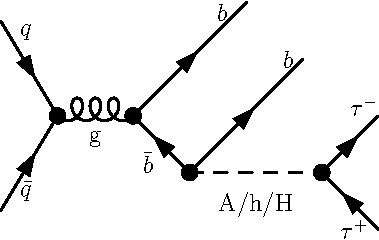
\includegraphics[height=3cm]{feyn_diagrams/diagrams/bbA3.pdf}
     }
     \subfigure[]{	
            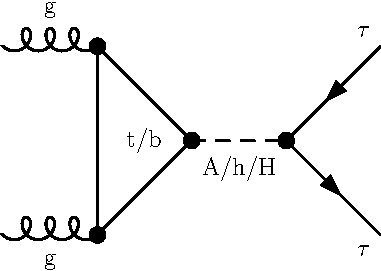
\includegraphics[height=3cm]{feyn_diagrams/diagrams/ggH.pdf}
	}	
     \end{center}
    \caption{Feynman diagrams for the production of the neutral MSSM Higgs bosons in association with  $b$-quarks (a,b,c) and via gluon fusion (d) 
	with subsequent decay into tau lepton pairs.}
   \label{fig:feyndiagSignal}
\end{figure}

The described signal topology  is common to several other  SM background  processes which in general  
have higher cross sections than the sought signal.
The dominant background processes are  $Z/\gamma^* \rightarrow \tau^+ \tau^- $ production
either via the  Drell-Yan process or in association with jets and  top quark production ($t\bar{t}$ and single top quark production ). 
Additional significant background contributions arise from  dibosons production 
($WW$, $WZ$, $ZZ$) and QCD multi-jet events with non-prompt leptons  from hadron decays.
Vector boson production ($\Wlnu$ or $\Zll$, where $\ell \equiv e,\mu$)  in association with jets 
is also considered, but has small impact on the total background contamination. Examples of 
leading order Feynman diagrams for the dominant background processes are shown in Figure~\ref{fig:feyndiagBack}.
The production cross sections times the branching fractions for signal and background processes are summarized in
Table~\ref{tab:MCxsec}. 
%The $W/Z$ and $b\bar{b}A/H/h$ production cross sections 
%are calculated to NNLO. The one for $\ttbar$, single top and dibosons cross sections are calculated at NLO.
%Finally, the direct $gg\rightarrow A/H/h$ signal cross sections 
%are calculated at NNLO and NLO for the top loop and the bottom loop respectively.
%

\begin{figure}[tp]
     \begin{center}
     \subfigure[]{		
            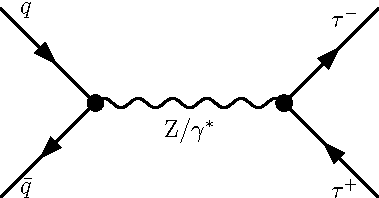
\includegraphics[height=3cm]{feyn_diagrams/diagrams/Ztautau.pdf}
     }\hspace{0.2cm}	
     \subfigure[]{		
            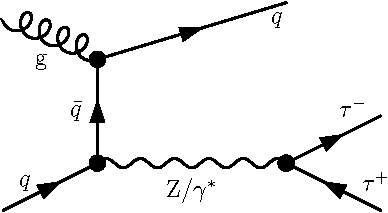
\includegraphics[height=3cm]{feyn_diagrams/diagrams/Z_plus_jet.pdf}
     }	
     \subfigure[]{		
            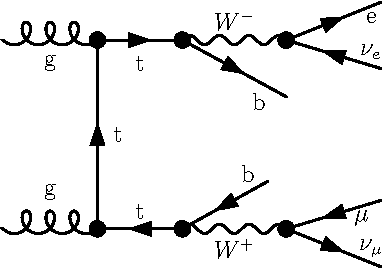
\includegraphics[height=3.5cm]{feyn_diagrams/diagrams/top.pdf}
     }\hspace{0.2cm}	
     \subfigure[]{	
            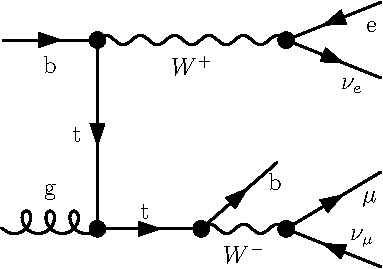
\includegraphics[height=3.5cm]{feyn_diagrams/diagrams/singletop.pdf}
	}	
     \subfigure[]{	
            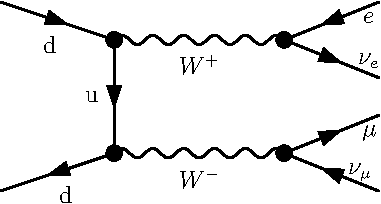
\includegraphics[height=3.2cm]{feyn_diagrams/diagrams/diboson.pdf}
	}\hspace{0.2cm}		
     \subfigure[]{	
            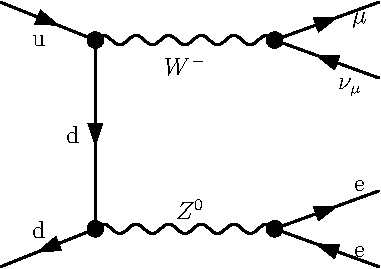
\includegraphics[height=3.2cm]{feyn_diagrams/diagrams/diboson2.pdf}
	}	
     \end{center}
    \caption{Examples of tree level Feynman diagrams for  the most important background processes. The production of 
	 $Z/\gamma^* \rightarrow \tau^+ \tau^- $, either via the Drell-Yan process or in association with jets,  is shown in (a) and (b)
	respectively, top quark pair and single top quark production in (c) and (d), while $WW$ and $WZ$ production in (e) and (f).
	}
   \label{fig:feyndiagBack}
\end{figure}


%The values of the steering parameters used for the HERWIG, JIMMY and PYTHIA
%generators are described in Ref.~\cite{ATLASMC09Tune}.

\begin{table}[!tp]
\begin{center}
\caption{The cross sections times by the relevant branching ratios~(BR) for signal and the considered
background processes, with $\ell= (e, \mu, \tau)$. 
Signal cross sections are calculated for the $m_{h}^{mod}$ scenario assuming
 $m_A=150$~GeV and $\tan\beta=20$. The masses of the other two neutral MSSM Higgs bosons are 
	in this case  $m_H=151$~GeV and $m_h=125$~GeV.} 
\vspace{2mm}
%\begin{footnotesize}
\begin{small}
\begin{tabular}{lr}
\hline \hline
Process                                                                 & Cross-section~$\times$ BR (pb) \\ [1pt]
\hline
\multicolumn{2}{c}{Signal ($m_A=150$~GeV, $\tan\beta=20$, $m_{h}^{mod}$ scenario) }  \\ [1pt]

$gg\rightarrow A/h/H \rightarrow\tau\tau \rightarrow e\mu+ 4\nu$                 &  $0.24 /0.20 / 0.95 $ \\
$pp \rightarrow b\bar{b}A/h/H \rightarrow \tau\tau \rightarrow e\mu + 4\nu$       & $0.53 /0.05 / 0.49   $ \\[1pt]
\hline
\multicolumn{2}{c}{Backgrounds} \\[1pt]
$W\rightarrow \ell \nu$+jets                           & 12.22$\times 10^3$ \\
$Z/\gamma^{*}\rightarrow \ell\ell$+jets       & 5.5$\times 10^3$ \\
$t\bar{t} \rightarrow \ell \ell + X$                                                              & 137.3 \\
Single top quark ($t-$, $s-$ and $Wt-$channels) $\rightarrow \ell + X$               & 28.4, 1.8, 22.4 \\
Dibosons (WW, WZ and ZZ ) $\rightarrow \ell \ell+ X$                                          & 20.6, 6.8, 1.55 \\ [1pt]
\hline 
\hline
\end{tabular}
\end{small}
 \label{tab:MCxsec}

\end{center}
\end{table}


\subsection{Analysis Strategy} \label{sec:strategy}


In this thesis, a search for the neutral MSSM Higgs boson decays
$A/h/H \rightarrow \tau^+ \tau^- \rightarrow e \mu +4\nu$ is presented. The $ee +4\nu$ and $\mu\mu +4\nu$ final states 
are not considered since  large background contributions are expected  from $\Zee$ and $\Zmumu$ decays,  respectively, 
such that the sensitivity of the search in these final
state is significantly reduced.

Candidate events are selected based on the topological properties of Higgs boson production
and decay. The  presence of exactly one electron and one muon is required in each event. The electron and the muon are required to be 
 isolated and of opposite electrical charge.
The  events are categorized into two orthogonal categories. In the so called  \emph{b-vetoed} event category,
the absence of b-tagged jets is required, 
thus searching mainly for the signal producion via gluon fusion. The main background 
process in  this category is $\Ztautau$. 
In contrast, the presence of exactly one  b-tagged jet is required in the so called \emph{b-tagged} event category, 
in which predominantly the signal producion in association with b-quark is searched for. The requirement of a b-jet 
in the final state suppresses the $\Ztautau$ background, consequently, $\ttbar$ and single top quark  production
are the main background processes in this event category. Further selection criteria are introduced in both event categories
optimised to enhance the signal wih respect to the background.

The  search is performed within the MSSM $m_h^{mod}$ benchmark scenario
scanning the $m_A - \tan\beta$ plane in the range $90 \leq m_A \leq 300$ GeV and $5 < \tan\beta < 60$.
The signal event yields and kinematical distributions are predicted by simulation.
The contribution of the dominant $\Ztautau$ background process is measured in a dedicated  signal-depleted control data sample
in order to reduce the systematic uncertainties of the simulation. Similarly, the QCD multi-jet background contribution 
is also estimated from a dedicated data control sample since this background process is hard to model. The
%the large cross section puts high demands on the number of simulated events.
contributions of  all  other background processes  are estimated by simulation.
The modelling of the background processes is  validated using different signal-depleted validation data samples where
good agreement is found.

Systematic uncertainties  on cross section calculations and the modelling of the detector response for 
simulated signal and background processes are taken into account. For background processes  determined from  data,
the uncertainties of the measurement methods are evaluated.

The statistical interpretation of the data is based on the 
comparison of the observed $\tau\tau$ invariant mass distributions with the predictions of the  background-only and signal-plus-background
hypotheses. Exclusion limits on the signal production are set by means of a binned profiled likelihood ratio
test statistic within the MSSM $m_{h}^{mod}$ scenario as constraints in the 
 $m_A - \tan\beta$ plane. Furthermore, the data are interpreted in a less model-dependent
way in terms of  upper limits on the cross section for the production of a generic Higgs boson $\phi$ with   mass  $m_\phi$ 
via the  processes $pp \rightarrow b\bar{b}\phi$ and $gg \rightarrow \phi$.


 

%neutral MSSM Higgs bosons with the ATLAS experiment at CERN is
%presented, using proton-proton collisions at centre-of-mass energy of
%8~TeV, with a recorded integrated luminosity of
%$20.3 \ifb$.



\subsection{Data and Simulated Event Samples}
\label{sec:sample}
\subsubsection{Data Sample}

The  presented results  are based on proton-proton collision data
recordered by the ATLAS experiment during 2012 at a centre-of-mass energy of $\sqrt{s}=8$~TeV
corresponding to an integrated luminosity of 20.3 fb$^{-1}$.
The events used in this analysis are recorded using a combination of a
single electroni trigger  and combined electron-muon triggers. Only events 
recordered with  all  relevant components of the ATLAS detector 
fully operational are considered.
Additional data quality requirements are applied according to~\cite{ATLASCLEANING}, rejecting 
events %with data corruption due to the LAr and Tile calorimeters and
with jet activity in known noisy calorimeter regions. 




\subsubsection{Signal Samples}
%Both the signal and background process modelled by Monte Carlo (MC)
%simulation were produced within the ATLAS MC12a production campaign.
%The generators used for the different processes are described below.
Signal production via the gluon fusion process $gg\rightarrow A/H/h$
was simulated with POWHEG~\cite{POWHEG} and the associated
$b\bar{b}A/H/h$ production with SHERPA~\cite{SHERPA}.  The
pseudo-scalar Higgs boson samples were generated in the mass range from
90~GeV to 300~GeV assuming $\tan\beta = 20$. Re-weighting of the production cross sections is applied 
to simulate other $\tan\beta$ values. All three  neutral Higgs bosons $A,h,H$ are assumed to decay 
with the same kinematical properties. The $m_h^{\mathrm{mod}}$ MSSM benchmark scenario is assumed
for the prediction of the mass and cross sections of the three neutral Higgs bosons for  given $m_A$ and $\tan\beta$ values.


\subsubsection{Background Samples}
The production of $W$ and $Z/\gamma^*$ bosons in association with jets
was simulated with the ALPGEN~\cite{Alpgen} generator. 
%This employs
%the MLM matching scheme~\cite{MLM} between the hard process,
%calculated with leading-order matrix elements for up to five jets, and
%the parton shower.  
The $t\bar{t}$ process was generated using the POWHEG program. Single top quark 
production via the  s-channel and via the   $Wt$ process was
 generated using MC@NLO~\cite{MCatNLO}, while single top quark production via 
t-channel  was generated with the AcerMC~\cite{AcerMC}.  Diboson processes ($WW$, $WZ$, $ZZ$) were generated with
 HERWIG~\cite{Herwig}.  For all ALPGEN  
and MC@NLO event samples described
above, the parton shower and hadronization were simulated with the  HERWIG
and the underlying event activity with the JIMMY~\cite{JIMMY} programme.
%The loop-induced $gg\rightarrow WW$ processes were generated using gg2WW~\cite{GG2WW}.  We are not using it Xsec very small
Different sets of parton density functions (PDFs)  are used depending on
the generator: CTEQ6L1~\cite{CTEQ6} is used with the ALPGEN and AcerMC while
CT10~\cite{CT10} is used with SHERPA, POWHEG and MC@NLO. 

TAUOLA~\cite{TAUOLA} and PHOTOS~\cite{PHOTOS} are used to model the
tau lepton decay and additional photon radiation from final state charged leptons
in the leading-log approximation, respectively.

The ATLAS detector response is simulated for all generated samples using the GEANT4~\cite{Geant4,ATLASSIM} package.
The reconstruction of physics objects, described in chapter~\ref{chap:obj}, is performed with the same software as used for 
the data.
The effects of simultaneous recording of additional proton collisions from the
same or neighbouring bunch crossings (pile-up) are taken into account in the detector
simulation. 



\section{Event Selection and Categorization}\label{sec:selection}


\subsection{The Common Selection Criteria}\label{sec:presel}

According to the kinematical properties of signal events, each event in data and simulation have to satisfy
the selection criteria described in the following. Since these are shared by both the b-tagged and the b-vetoed event category,
they are referred to as common selection criteria:


\begin{enumerate}[label=(\roman*)]
\item The trigger selection requires the presence of a single electron with $\pt > 24$ GeV or, alternatively,
	an electron with  $\pt > 12$ GeV togheter with a muon with  $\pt > 8$ GeV. 

\item At least one reconstructed vertex with more that three associated tracks in order to 
	reject background from cosmic muons.

\item Exactly one reconstructed ``Tight'' electron with $|\eta| < 1.37 $ or $1.52 < |\eta| < 2.47$ and
	 $\pt > $ 15 or 25~GeV, depending on the trigger that selected the event. 

\item Exactly one ``Combined'' muon with $|\eta| < 2.5$ and  $\pt > $ 10~GeV.

\item The electron have to be isolated with $E_T^{cone}/ \pt < 0.08$ and $P_T^{cone}/ \pt < 0.06\,.$ 

\item The muon have to be isolated with  $E_T^{cone}/ \pt < 0.04$ and $P_T^{cone}/ \pt <  0.06\,.$ 

\item Muon and electron have to be of opposite charge.

\item Removal of overlap between reconstructed electron, muon, $\tau$-jets and jets is performed.

\item The event is rejected if at least one hadronic $\tau$ lepton decay is found with  $\tau$-jet transverse 
	momentum  $\pt > $ 15 GeV. $\tau$-jets candidate are required to be associated to one or three charged tracks,
	for the identification a ``Medium'' BDT working point is chosen, additionally, a BDT-based electron veto is 
	applied. 

\item To reduce QCD multi-jet background contamination, the invariant mass of electron and muon has to be 
	greater than 30 GeV.

\end{enumerate}
Details on  the definition of physics objects and the applied quality criteria  can be found in  chapter~\ref{chap:obj}.

Events accepted by the common selection criteria are divided into \emph{b-tagged} and \emph{b-vetoed}  categories by requiring the presence 
or the absence, respectively, of exactly one b-tagged jet  in the event. A jet is tagged  ad a b-jet if  has 
$\pt > 20$ GeV, $|\eta| < 2.5$, $\text{JVF} > 0.5$ and if it passes  the $MV1$ b-tagging criteria corresponding to 
70\% of b-quark efficiency $\epsilon_b^{\ttbar}$ in $\ttbar$ events. Further selection criteria
are applied to each category and optimized separately as described in the following.

\subsection{b-Vetoed Event Category}\label{sec:veto}
%\subsection{Selections}

%The final state of Higgs decaying into tau pair coincide with the one from  
A veto on the presence of b-tagged jets in the final state allows for the selection of signal events
produced predominantly via gluon fusion. In this event category, the 
$\Ztautau$  process is an irreducible background due to the same topology of the Higgs and $Z$ boson decay.
Other background processes can  be discriminated from the signal due to their kinematical properties.
The $\tau$ leptons from the Higgs boson decay are highly boosted and so are their decay products, resulting
in significantly different lepton kinematics in the Higgs decays than in  diboson or $\ttbar$ background processes. 
Firstly, the electron and muon from Higgs boson decay are predominantly 
emitted back-to-back as illustrated in Figure~\ref{dphi} which shows
the angular distance $\Delta\phi_{e,\mu} = |\phi_{e} - \phi_{\mu}|$  between the two leptons in the transverse plane 
for the signal and background processes. Secondly, the neutrinos from Higgs boson decay  are predominantly
collinear with the charged leptons. Thus, the angular correlation between the direction of the missing transverse energy 
and the two charged leptons in the transverse plane, 
%re can be mathematically seen as the sum of scalar product between missing energy and the leptons four-vectors in the
%transverse plane, if the vectors are normalised to unit versors then what remains is a relation only between angles:
$$ \hat{E}_{T}^{miss} \cdot ( \hat{P}_{T}^{\mu} + \hat{P}_{T}^{e} ) = cos(\Delta\phi_{E_{T},\mu}) 
+ cos(\Delta\phi_{E_{T},e}) = \sum_\ell cos(\Delta\phi_{E_{T},\ell}) \,,$$
tends to zero as shown in Figure~\ref{sumcosphi}. 
These two features are used to discriminate between  signal and the W boson, top quark and  dibosons background processes.
%ck-to-back and the neutrinos not collinear with them.
%In b-vetoed category these two variables are sufficient to suppress contribution from dibosons,
No further selection criteria are applied in the b-vetoed category, since  no significant improvement
in signal sensitivity could be achieved.
The described selection criteria are listed in Table~\ref{tab:sel}, while in Table~\ref{tab:eventsel:bveto}
the predicted numbers of signal and background events after each selection stage  are shown.


\begin{table}[!t]
  \begin{center}
   %\begin{footnotesize}	
    \caption{Summary of the event selection criteria in the b-tagged and b-vetoed event categories applied after the common 
	event selection has been performed.}
    \begin{tabular}{p{4cm}c}
      \hline \hline
      Category & Selection \\ [3pt]
      \hline
%      Common Selection 	&  Trigger \\
%	&	At least one reconstructed vertex with $> 3 $ tracks \\
%	& 	Exactly one tight isolated electron with $\pt > 15 $ or 25 GeV  \\
%	&	Exactly one Combined isolated muon with  $\pt > 10$ GeV \\
%	& 	Opposite charge between electron and muon \\ 
%	&	Overlap removal\\
%	&	Tau Veto \\
%	&	$M_{e-\mu} > 30$ GeV \\
%      \hline
      b-vetoed &  No b-tagged jets \\	
      & $\Delta\phi_{e,\mu}>1.6$ \\
      & $\sum\cos\Delta\phi_{E_{T},\ell} > -0.4$ \\[5pt]
      \hline
      b-tagged & Exactly one b-tagged  jet \\
      & $\Delta\phi{e,\mu}>2$ \\
      & $\sum\cos\Delta\phi_{E_{T},\ell} > -0.2$ \\
      & $ H_T < 100$ GeV \\
      & $P_{T\mu} + P_{Te} + \met < 100$ GeV \\[3pt]
      \hline \hline
    \end{tabular}
    \label{tab:sel}
  %\end{footnotesize}
  \end{center}
\end{table}

\begin{figure}[p]
     \begin{center}
     \subfigure[]{		
            \includegraphics[page=16,width=0.47\textwidth]{figure/final_plots/presel_total_final.pdf}
            %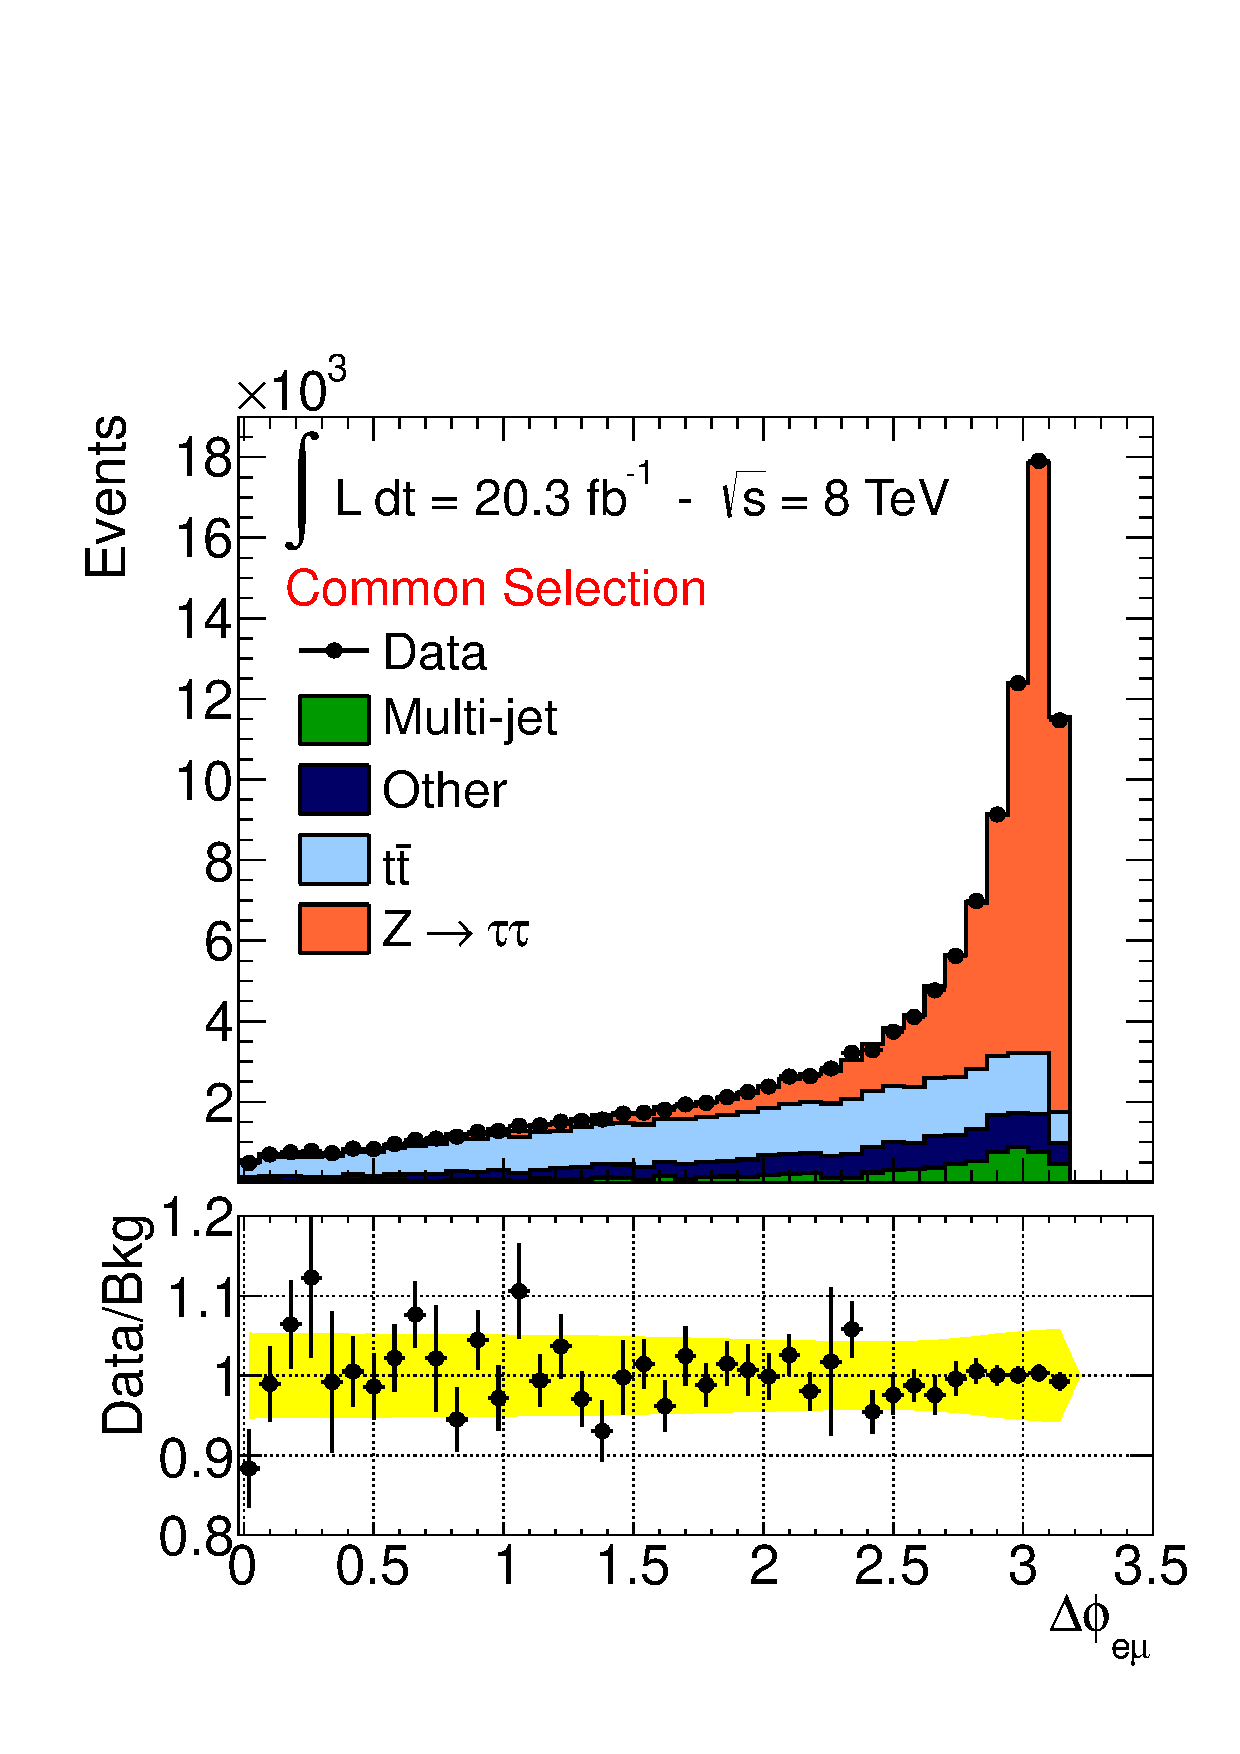
\includegraphics[width=0.47\textwidth]{figure/final_plots/std_presel_deltaPhi.pdf}
	    \label{dphi}	
     }	
     \subfigure[]{		
            \includegraphics[page=20,width=0.47\textwidth]{figure/final_plots/presel_total_final.pdf}
            %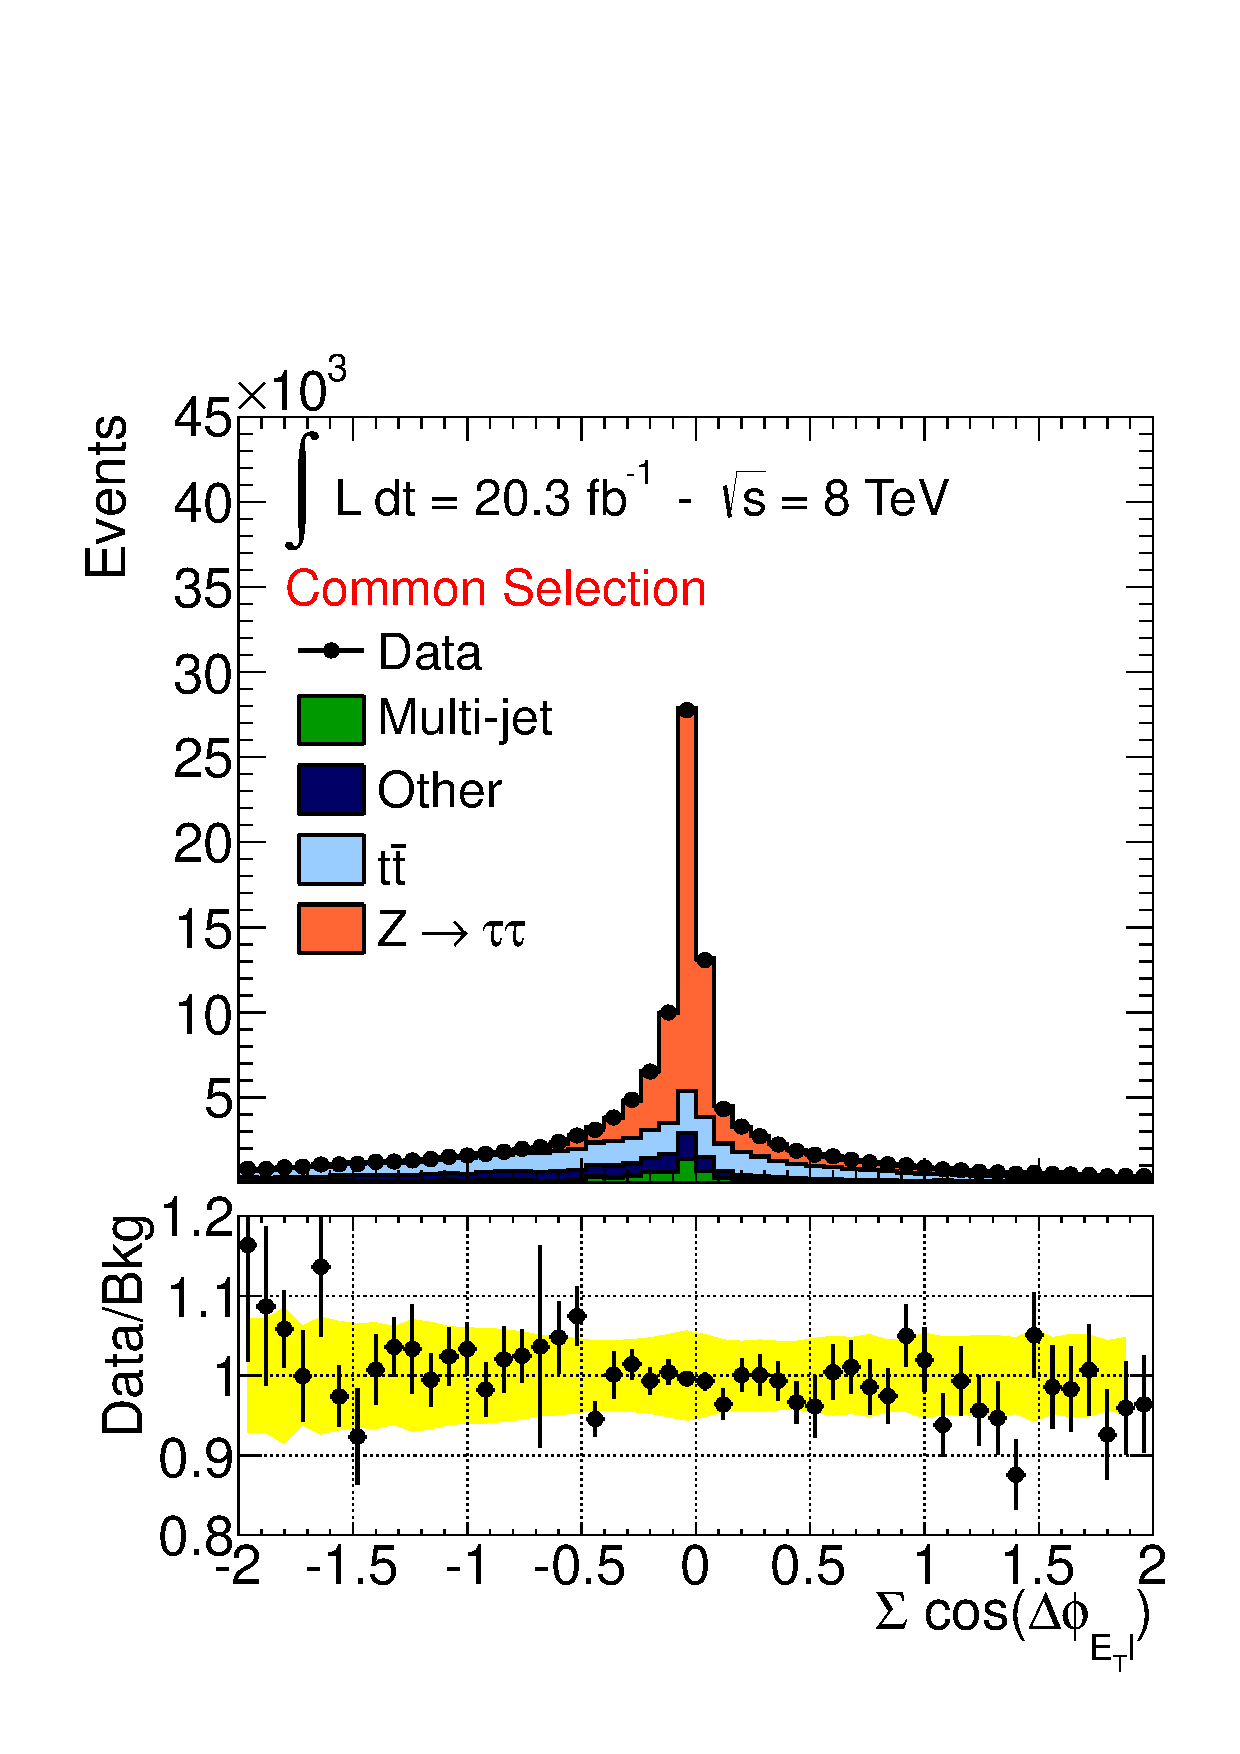
\includegraphics[width=0.47\textwidth]{figure/final_plots/std_presel_sum_cos_deltaPhi.pdf}
	    \label{sumcosphi}	
     }	
     \subfigure[]{		
            \includegraphics[page=19,width=0.47\textwidth]{figure/final_plots/presel_total_final.pdf}
            %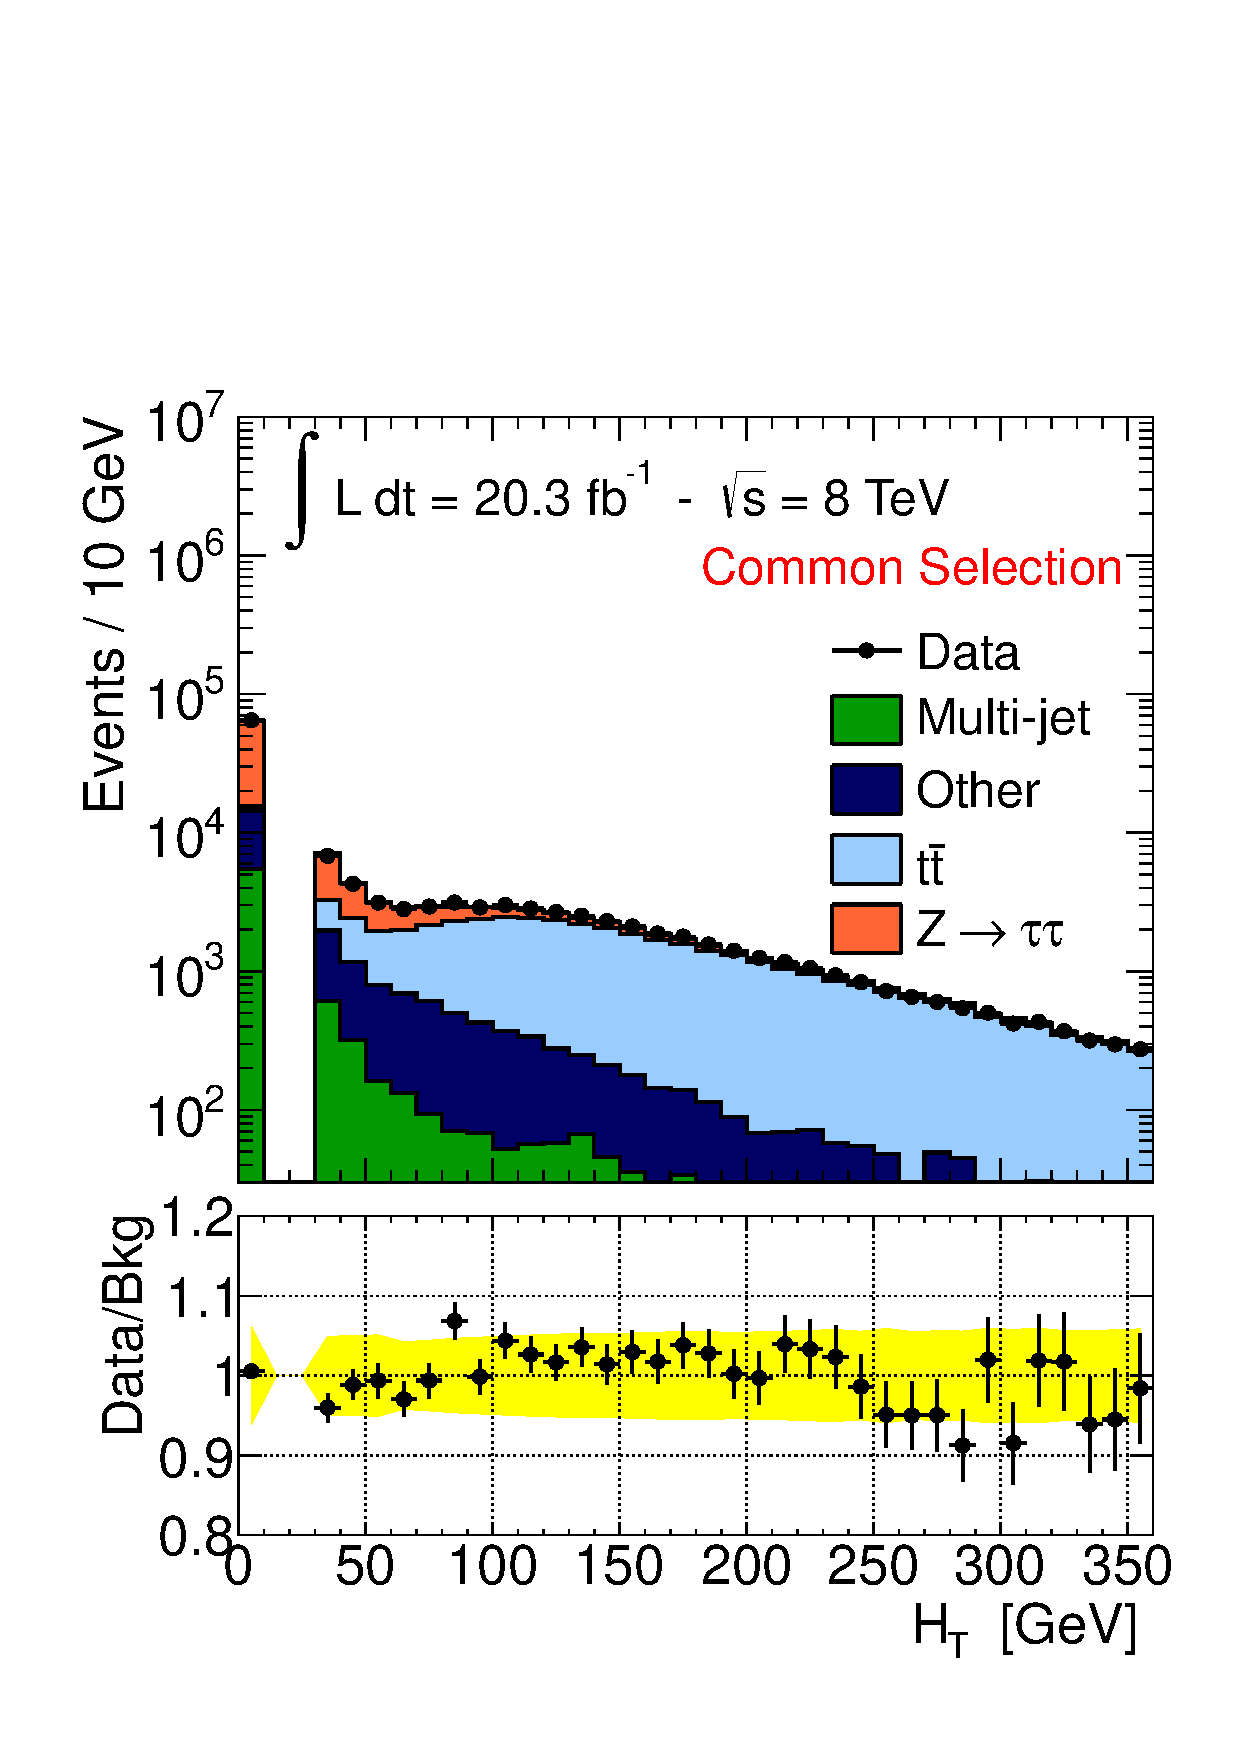
\includegraphics[width=0.47\textwidth]{figure/final_plots/std_presel_Ht.pdf}
	    \label{Ht}	
     }	
     \subfigure[]{		
            \includegraphics[page=12,width=0.47\textwidth]{figure/final_plots/presel_total_final.pdf}
            %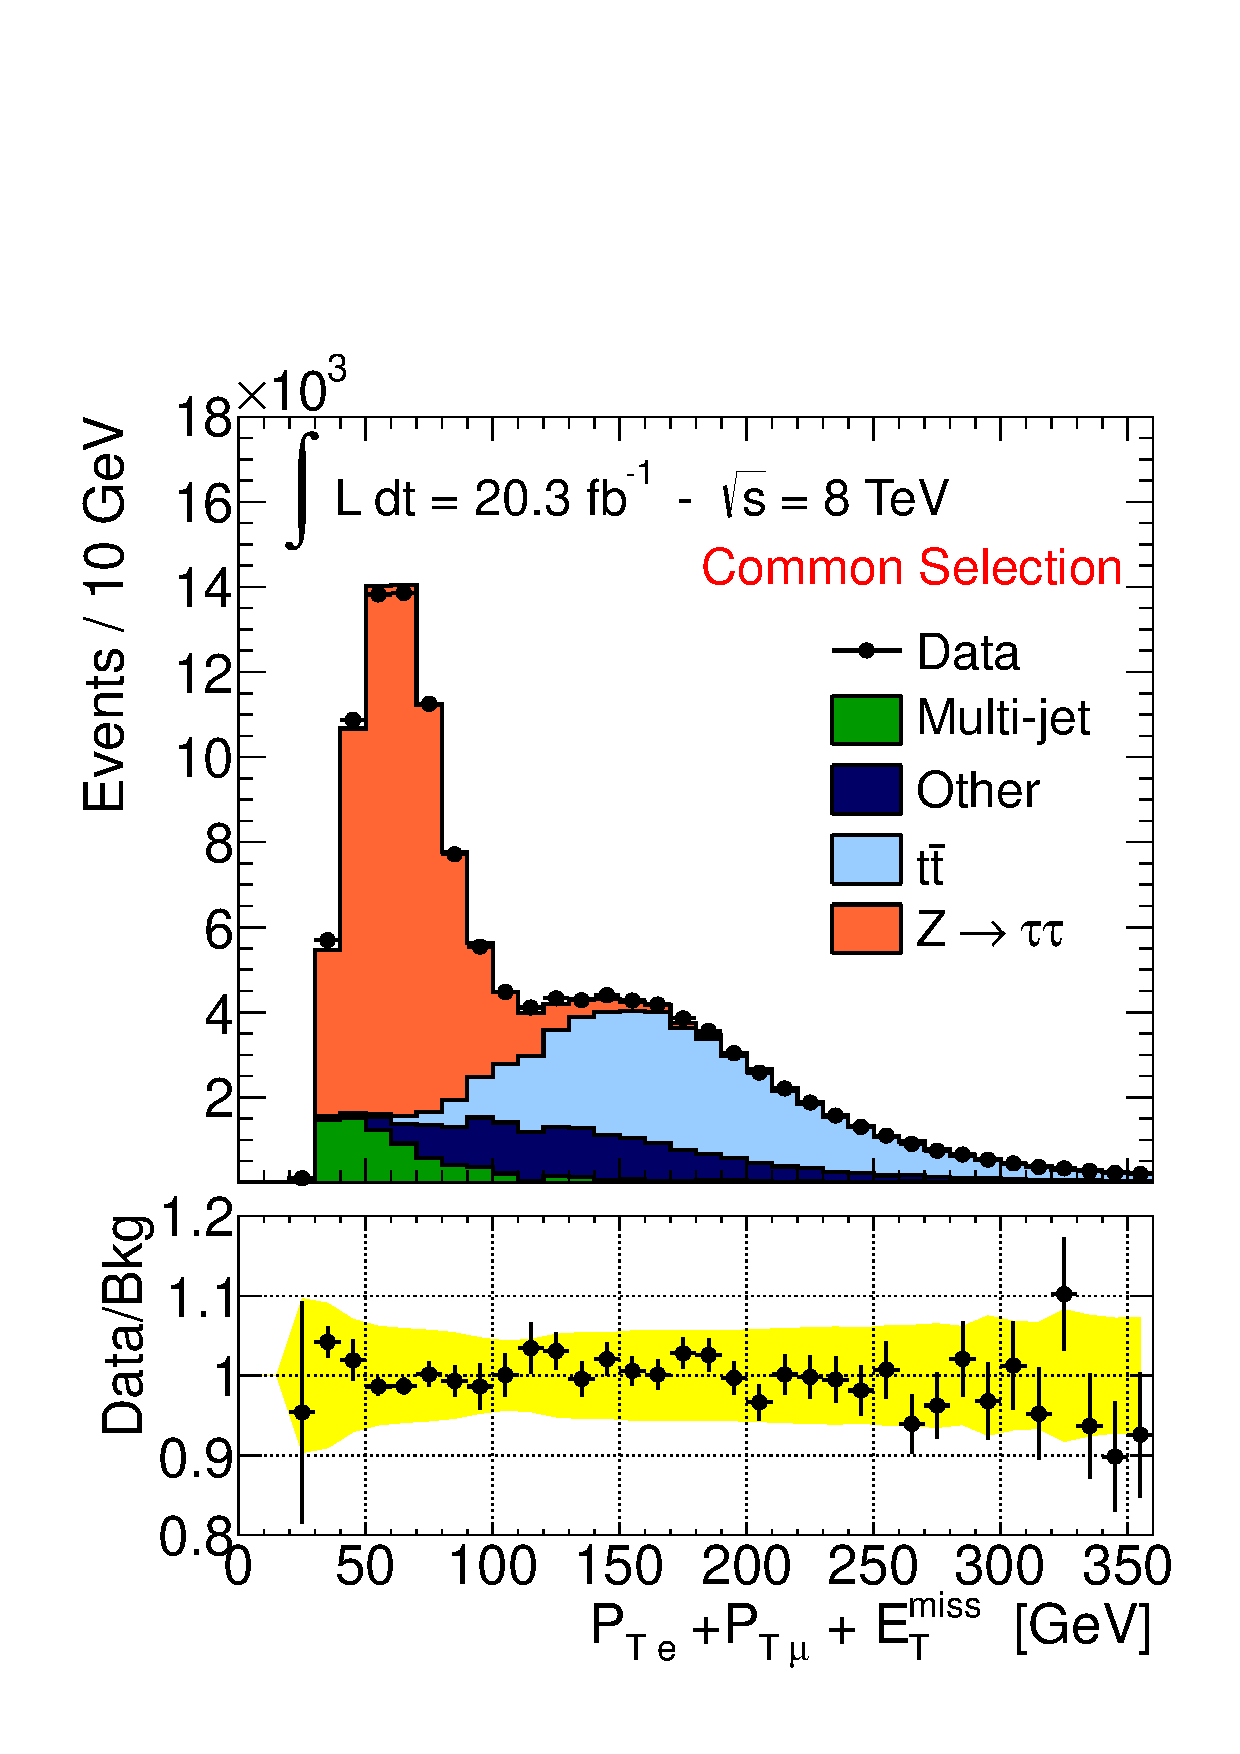
\includegraphics[width=0.47\textwidth]{figure/final_plots/std_presel_Et_plus_leptonPt.pdf}
	    \label{sumlepPt}	
     }	

    \end{center}
    \caption{Distributions of discriminating variables electron-muon angualar separation
	$\Delta\phi{e,\mu}$ (a), the angular correlation between charged lepton and $\met$ $\sum\cos\Delta\phi_{E_{T},\ell}$ (b),
	the total sum of jet $\pt$ (c), the sum of charget lepton $\pt$ and $\met$ (d), after the common selection has been applied.
 	The notation ``Other'' stands 	for the electroweak processes $\Wlnu$, $\Zll$, diboson and single top quark production.
	The prediction for the background contributions is determined as described in 	Section~\ref{sec:BackgroundEstimation}.
	The superimposed signal is obtained assuming the $m_h^{mod}$ scenario for $m_A=150$~GeV and $\tan\beta=20$ and it is scaled
	by a factor ten. The error bars on the ratio of observed and predicted events represent the statistical uncertainty on data,
	whereas the yellow and red band indicates the systematic and statistical uncertainty on the background prediction (see Section~\ref{sec:Systematics}),
	respectively.}
   \label{fig:selections}
\end{figure}

\subsection{b-Tagged Event Category}\label{sec:tag}
The requirement of exactly one b-tagged jet in the b-tagged event category predominantly selects signal events produced 
where the Higgs bosons are produced in  association with b-quarks.
Background processes with b-jets, as the $\ttbar$ and single top quark production, are enhanced compared to the $\Ztautau$ background.
Also in this category requirements on $\Delta\phi_{e,\mu}$ and $\sum\cos\Delta\phi$  are imposed to reduce the top quark and diboson background contributions
as described for the b-vetoed event category. Further selection criteria specific for the b-tagged category
are employed  as described below.

Signal events in this event category can be discriminated from  top quark given their relatively low jet activity. 
The $\ttbar$ events are likely to have two or more highly enegetic reconstructed jets, unlike the signal
b-jets which have relatively low energy. Low jet activity is ensured by requesting the sum of the jet transverse momenta $H_T$ to be small.
The $H_T$ distribution is shown in Figure~\ref{Ht}. The jets used for the calculation of $H_T$  have 
to fullfill $\pt > 30 $ GeV, $|\eta| < 4.5$  and $\text{JVF} > 0.5 $ (if $|\eta| < 2.5$).

Another feature that discriminates top quark  pair production from the Higgs boson signal is the higher invariant mass 
of the decay products of the former as the highest Higgs mass considered in this  search is 300 GeV.
The sum of the electron and muon transverse momenta and of  \met is  used as 
discriminating variable and is shown in Figure~\ref{sumlepPt}$\,.$

The optimized selection criteria for the b-tagged event category are shown in Table~\ref{tab:sel}.
In Table~\ref{tab:eventsel:btag} the predicted numbers of signal and background events after each selection stage are given in 
 the b-tagged event category.






\subsection{Mass Reconstruction with the MMC Technique}\label{sec:mmc}

Acurate invariant mass reconstruction of a di-$\tau$ resonance is a challenging task due to the undetected neutrinos. 
In this analysis there are a total of four neutrinos in the final state, two from  each 
of the $\tau$ lepton decays.
% In case of leptonic decay of the $\tau$ leptons
%a total of four neutrinos are involved in the final state. 
The invariant mass depends on eight unknown which are the components of the total neutrino four-momenta 
in each of the $\tau$ lepton decays. These unknowns are  constrained by the two measured component of the 
 missing transverse energy $\vec{E}_T^{miss}$ and by  the $\tau$ lepton mass $M_{\tau}$ via the following four equations:
% 
%In case of leptonic decay of both $\tau$ leptons a pair of neutrinos for each
%of them are involved in the final state,  the system presents then eight unknowns, which corresponds to the four-momentum of the neutrinos pairs.
%Four additional kinematic constraint are set by the following equations:
%There are four additional constraint 
%which come from the measurement of \MET and from the fact that each single decay should have invariant mass equal to the tau mass:
\begin{equation} \label{eq:MMC}
\begin{split}
%\begin{align}
%\begin{gather*}  
&\vec{E}_T^{miss} = \vec{P}_{T}^{mis_{1}} +  \vec{P}_{T}^{mis_2} \,,\\
&M_{\tau_{i}}^2 = m^2_{mis_{i}} + m^2_{vis_{i}} + 2 \mathbf{P}_{vis_i} \cdot \mathbf{P}_{mis_i} \,, \\
%\end{align}
%\end{gather*}
\end{split}
\end{equation}
where \emph{i}=1,2 distinguish the two $\tau$ leptons.
$\vec{P}_{T}^{mis_{i}}$, $m_{mis_{i}}$ and $\mathbf{P}_{mis_{i}}$ are the transverse momentum vector, the invariant mass and 
the four momentum of the neutrino pair originating from the decay of the $i$-th  $\tau$ 
lepton. $\mathbf{P}_{vis_i}$ and $m_{vis_{i}}$ are the known four momenta and mass of the charged lepton from the $i$-th $\tau$ lepton decay.
The remaining four degrees of freedom can be 
further constrained, assuming for example that the neutrinos are collinear with the electron or muon from the same 
$\tau$ lepton decay. This so-called collinear approximation, however, leads to  rather limited  mass resolution.

\begin{table}[!tp]
  \centering
   \begin{footnotesize}	
  \begin{tabular}{ccccc}
    \hline\hline
	&	Common Selections			&	n(b-jet)=0			&	$\Delta\phi(e-\mu)>1.6$			&	$\sum\cos\Delta\phi > -0.4$ 		\\	
    \hline
   \hline
Data	&	125886			&	89155			&	-			&	-				-			\\
   \hline
Multi-jet	&	6693	$\pm$	456	&	6357	$\pm$	461	&	5322	$\pm$	438	&	4137	$\pm$	339	\\
\Zll 	&	569	$\pm$	48	&	564	$\pm$	48	&	516	$\pm$	47	&	434	$\pm$	44		\\
\Wlnu	&	1625	$\pm$	155	&	1604	$\pm$	155	&	1145	$\pm$	125	&	714	$\pm$	101		\\
Dibosons	&	9338	$\pm$	48	&	9235	$\pm$	48	&	7358	$\pm$	43	&	4002	$\pm$	31		\\
\ttbar	&	40632	$\pm$	106	&	7707	$\pm$	46	&	5044	$\pm$	37	&	3416	$\pm$	31		\\
Single Top	&	4449	$\pm$	44	&	1664	$\pm$	27	&	1124	$\pm$	22	&	682	$\pm$	18	\\
\Ztautau	&	61503	$\pm$	68	&	60440	$\pm$	67	&	58078	$\pm$	65	&	55303	$\pm$	64	\\
%Signal	&				&				&	-			&	-						\\
    \hline
  \end{tabular}
  \caption{Number of observed and predicted signal and background events, after each selection stage in the b-vetoed event category.}
  \label{tab:eventsel:bveto}
   \end{footnotesize}	
\end{table}

\begin{table}[!t]
  \caption{Numbers of observed and predicted signal and background events after each selection stage in the b-tagged event category.}
  \centering
   \begin{footnotesize}	
  \begin{tabular}{cccccccc}
    \hline\hline
	& 	n(b-jet)=1			&	$\Delta\phi$&	$\sum\cos\Delta\phi$			&	$P_{T\mu} + P_{Te} + \met$&	$ H_T$	\\
   \hline
Data	&	23352			&	-			&	-			&	-			&	-						\\
   \hline
Multi-jet	330	$\pm$	40	&	208	$\pm$	27	&	135	$\pm$	22	&	114	$\pm$	17	&	100	$\pm$	15	\\
\Zll 	&	5.2	$\pm$	1.8	&	2.3	$\pm$	1.1	&	2.3	$\pm$	1.1	&	1.7	$\pm$	1.0	&	0.9	$\pm$	0.8		\\
\Wlnu	&	20	$\pm$	6	&	15	$\pm$	6	&	13	$\pm$	6	&	10	$\pm$	6	&	10	$\pm$	6		\\
Dibosons	&	99	$\pm$	5	&	63	$\pm$	4	&	36.4	$\pm$	3.0	&	14.8	$\pm$	1.8	&	13.3	$\pm$	1.8		\\
\ttbar	&	19810	$\pm$	70	&	9680	$\pm$	50	&	6450	$\pm$	50	&	808	$\pm$	15	&	350	$\pm$	10		\\
Single Top &	2456	$\pm$	33	&	1223	$\pm$	23	&	784	$\pm$	18	&	122	$\pm$	7	&	99	$\pm$	7		\\
\Ztautau &	952	$\pm$	9	&	625	$\pm$	7	&	540	$\pm$	7	&	482	$\pm$	6	&	421	$\pm$	6		\\
%Signal		&				&	-			&	-			&	-			&	-						\\
    \hline
    \hline
  \end{tabular}
  \label{tab:eventsel:btag}
   \end{footnotesize}	
\end{table}  %INCOMPLETE ------------missing signal

In this analysis, the so-called "Missing Mass Calculator" (MMC) algorithm
is used to determine the most likely  invariant mass of the di-$\tau$ system for a given event topology. %event kinematics
The implementation of the MMC method in this search is based on~\cite{MMC}. 
The MMC algorithm solves the equations~\ref{eq:MMC} for a set of grid points in a 
%assigning values to the yet undetermined variables, performing a ``scan'' over a 
four-dimensional parameter space. The four independent  variables are chosen 
to be $ m^2_{mis_{i}}$ and $cos\theta^*_i$. Where $\theta^*_i$ is 
the angle between the $\tau$ lepton and the charged lepton originating from its decay.
The di-$\tau$ invariant mass in each  event is   calculated for each grid point of the parameter space.
Each solution is weighted by the probability for that parameter configuration determined by Monte Carlo 
simulation using the PYTHIA generator supplemented by the TAUOLA package. 
The invariant mass \mmc of the di-$\tau$  system is then estimated  as the maximum of the weighted invariant 
mass distribution from all grid points.

\begin{figure}[p]
     \begin{center}
     \subfigure[]{		
            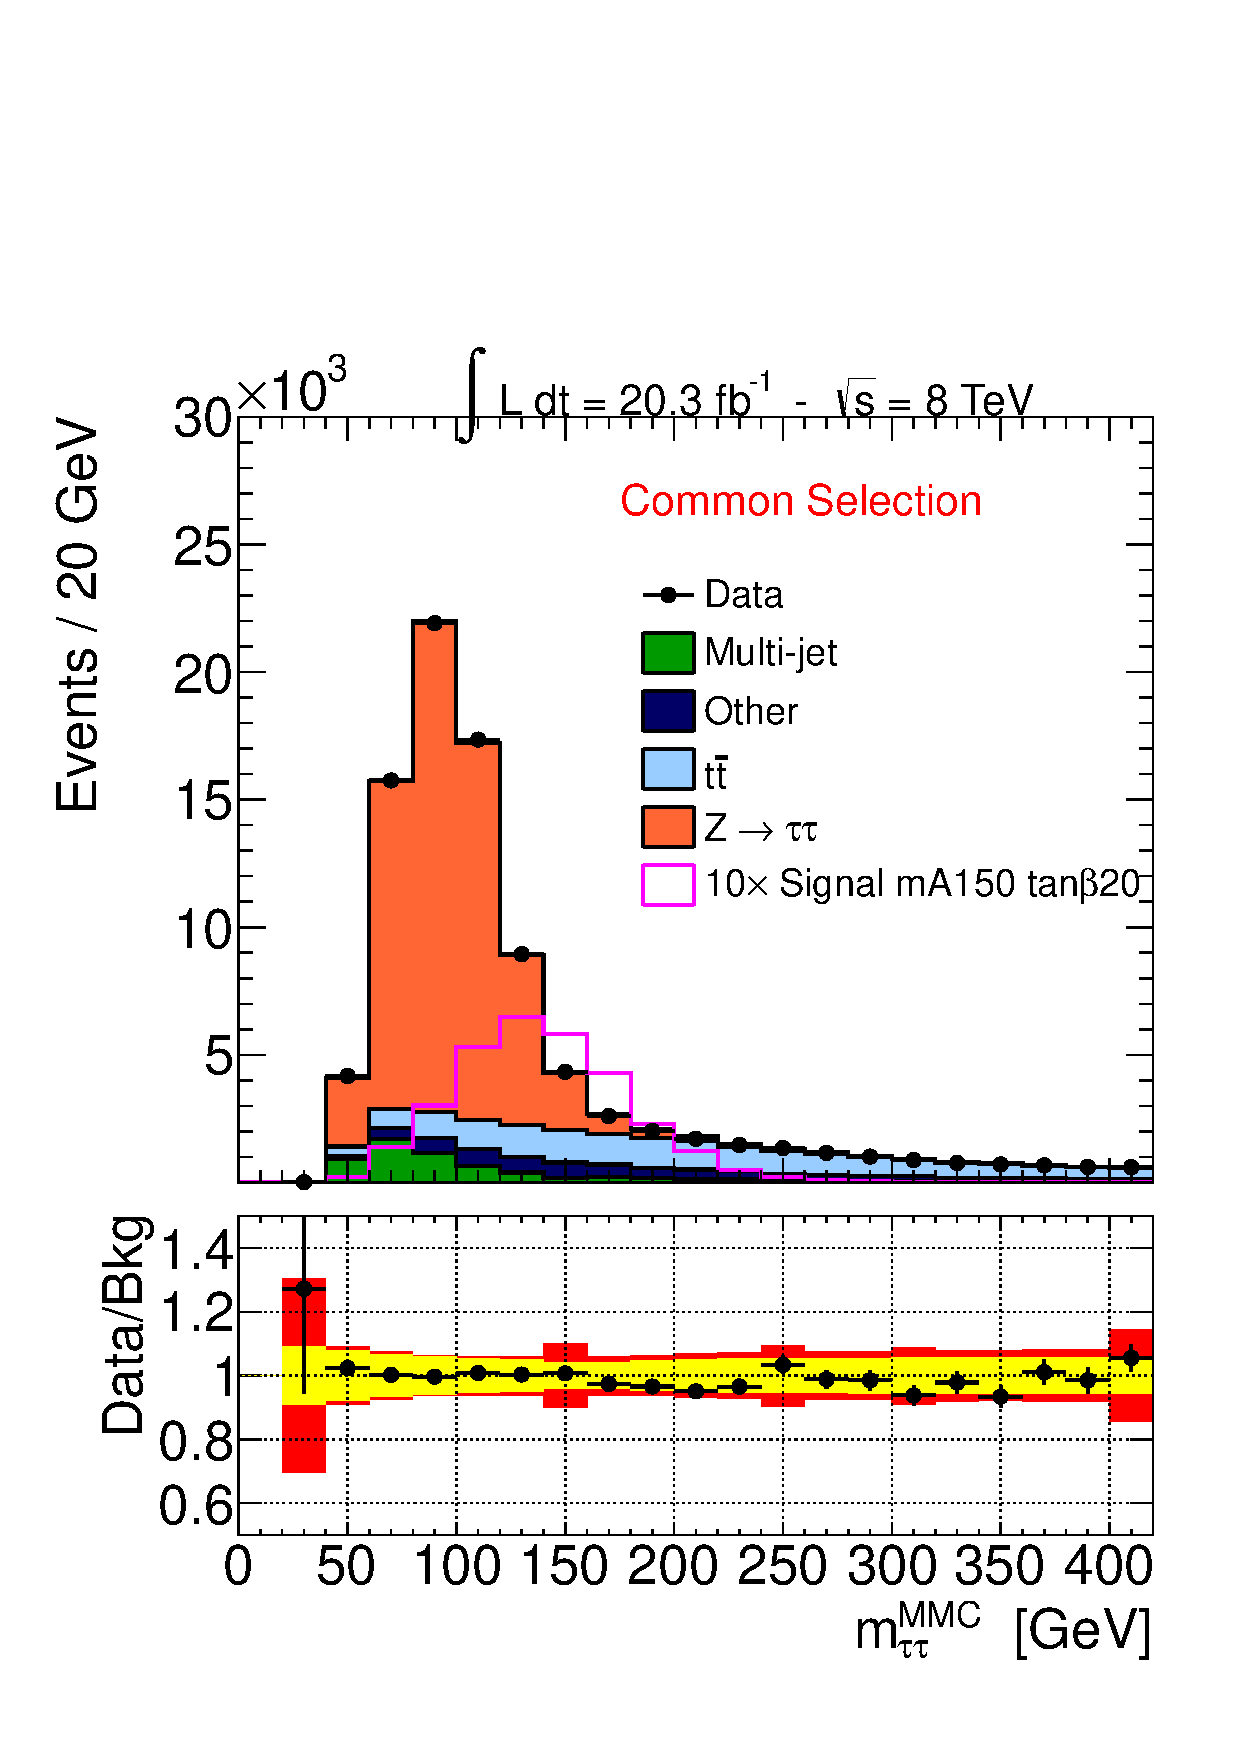
\includegraphics[page=1,width=0.47\textwidth]{figure/final_plots/presel_total_final.pdf}
            %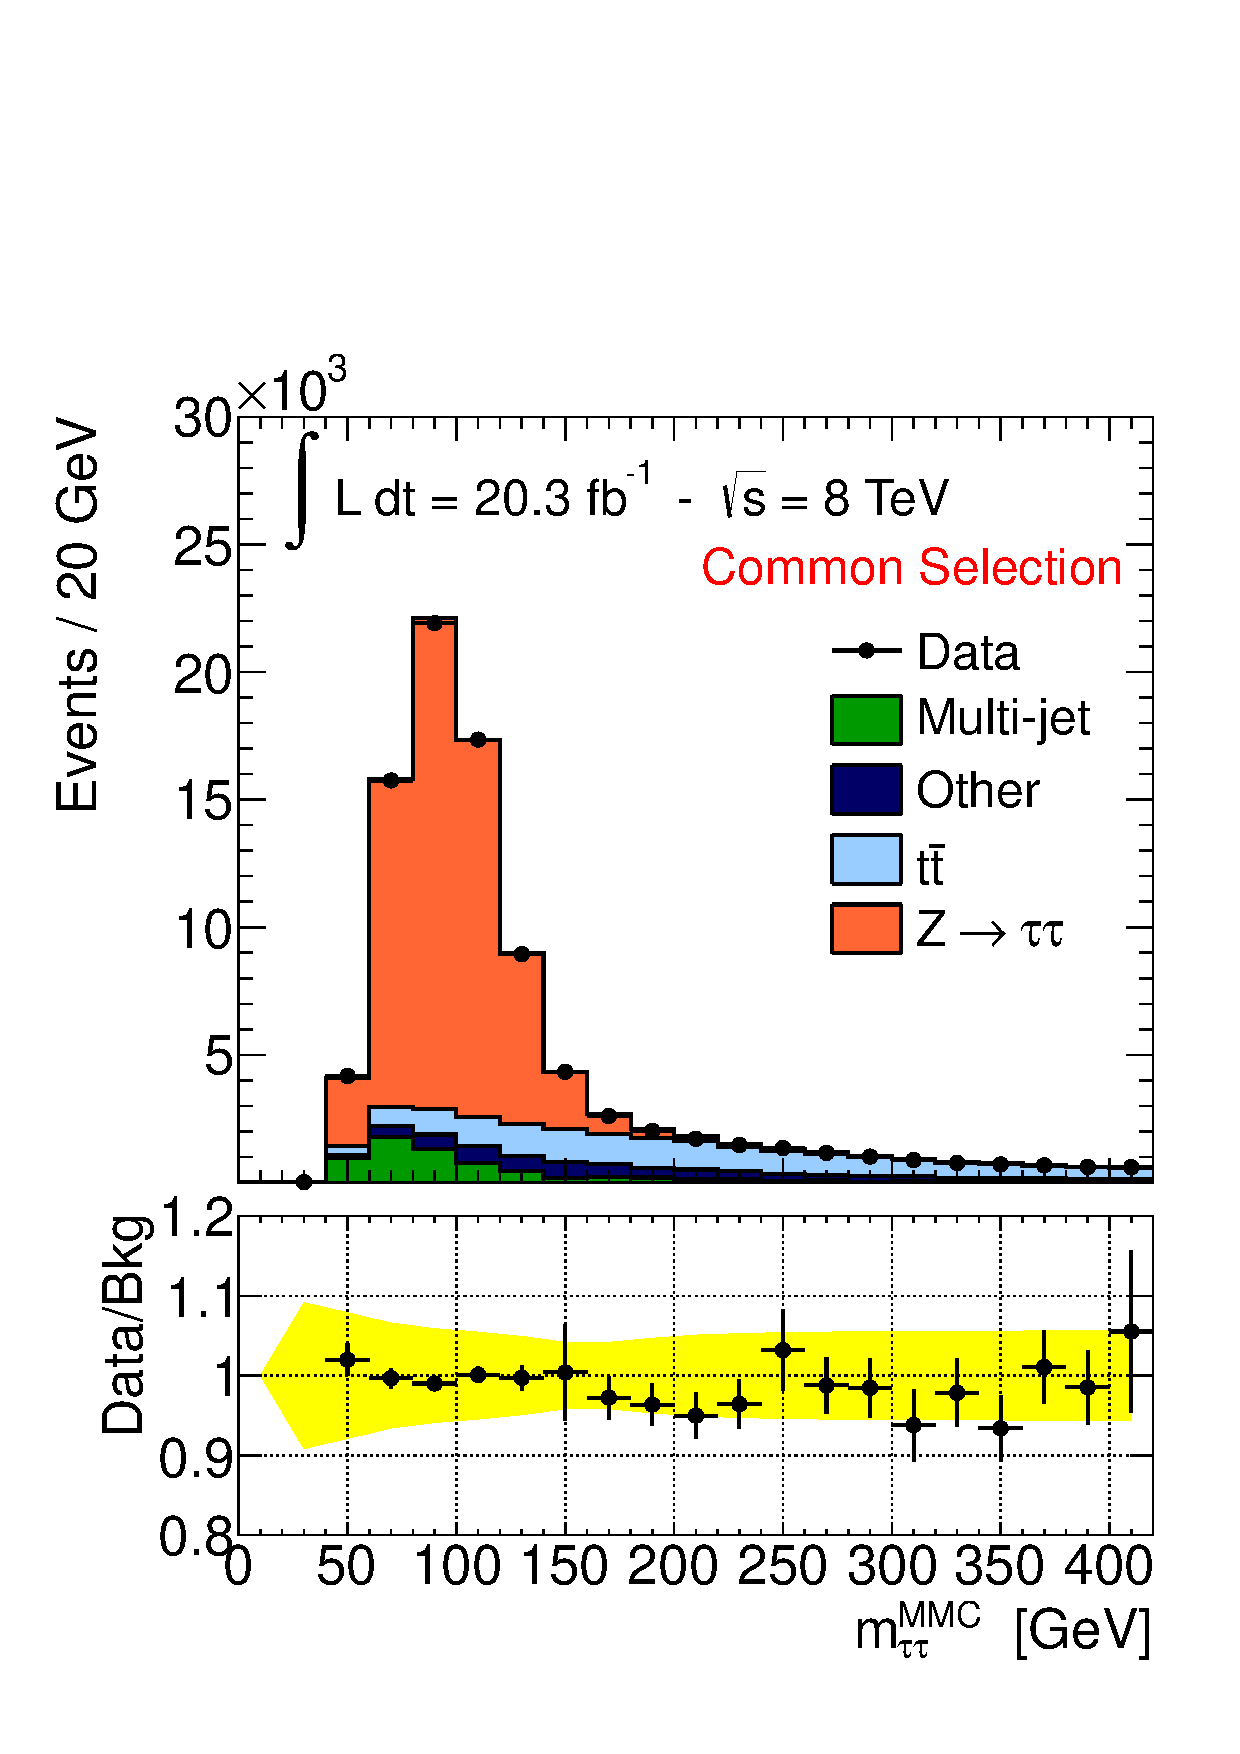
\includegraphics[width=0.47\textwidth]{figure/final_plots/std_presel_mmc_mass.pdf}
     }	
     \subfigure[]{		
            \includegraphics[page=17,width=0.47\textwidth]{figure/final_plots/presel_total_final.pdf}
            %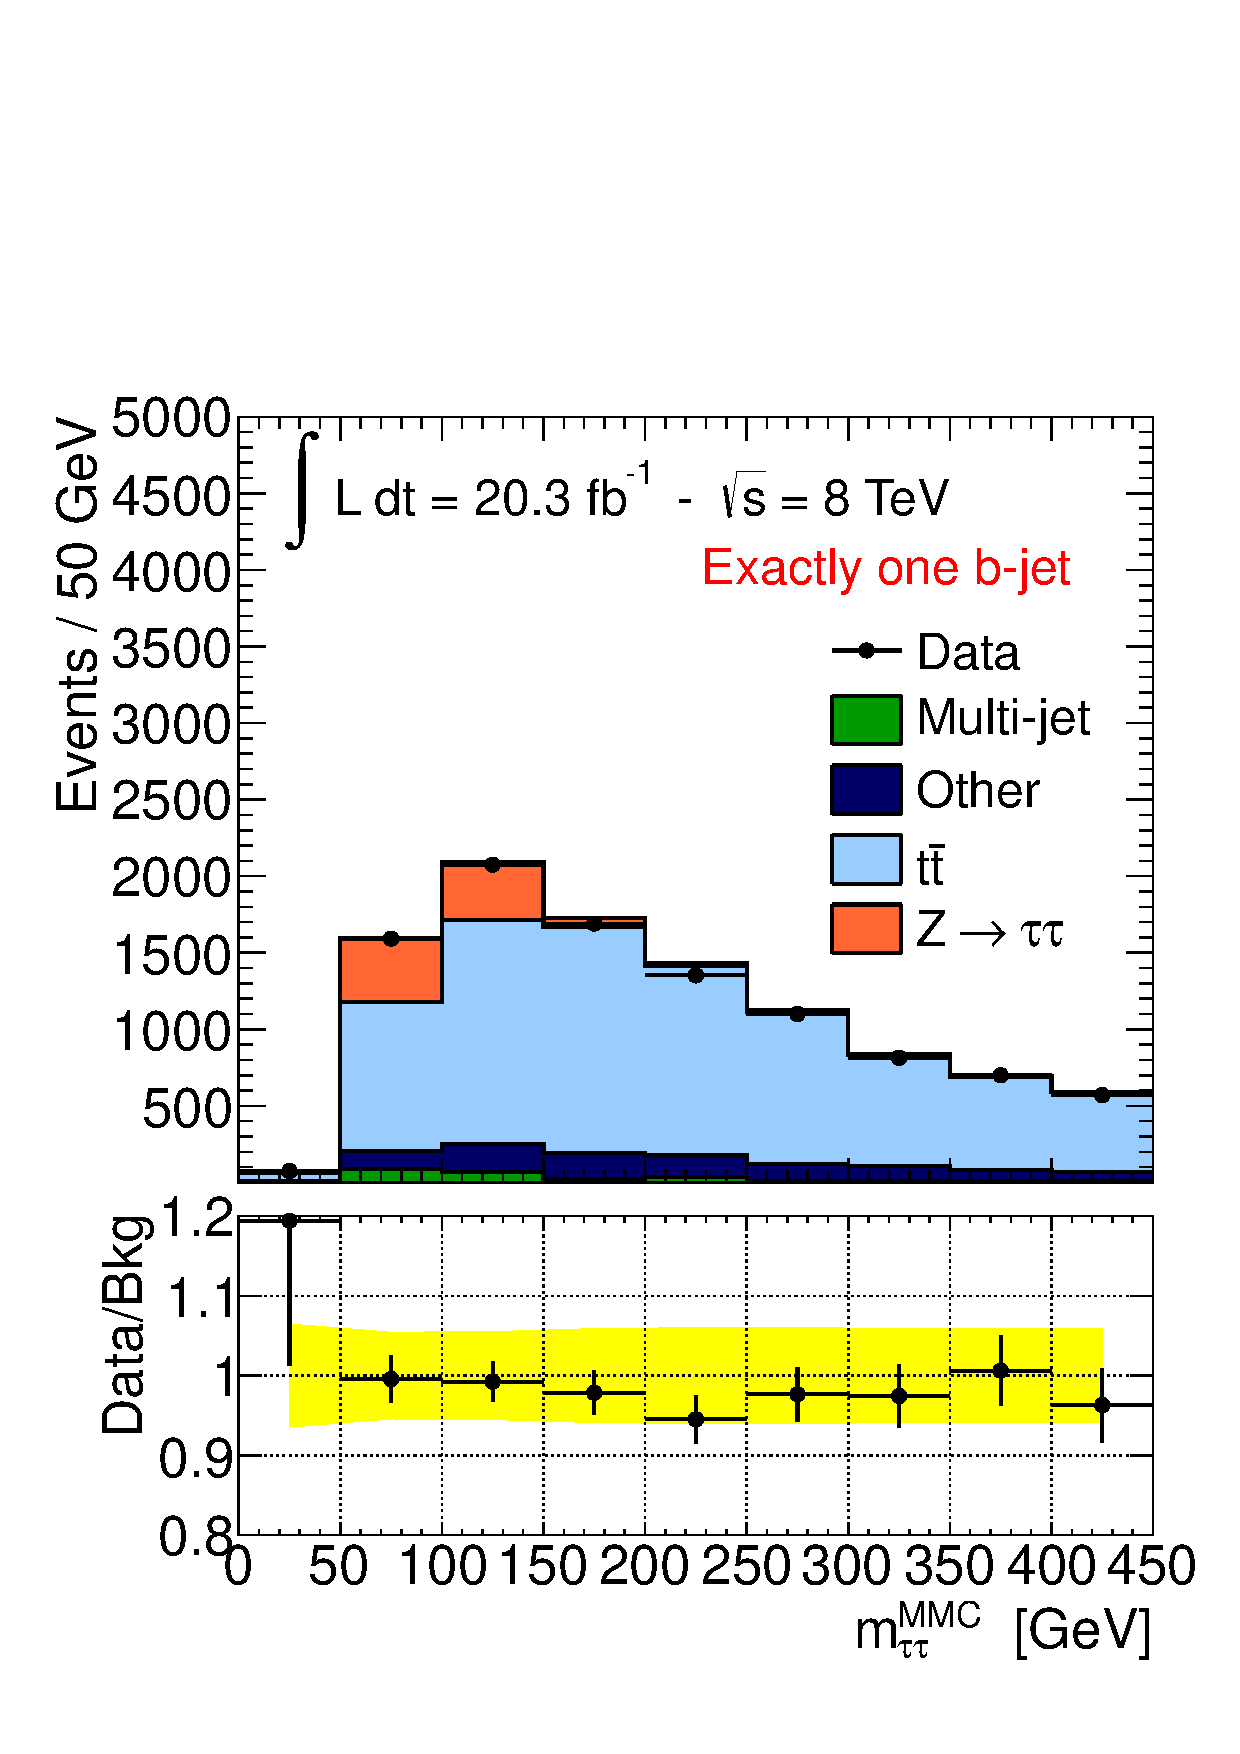
\includegraphics[width=0.47\textwidth]{figure/final_plots/std_presel_Btag_mmc_mass.pdf}
     }	
     \subfigure[]{		
            \includegraphics[page=2,width=0.47\textwidth]{figure/final_plots/presel_total_final.pdf}
            %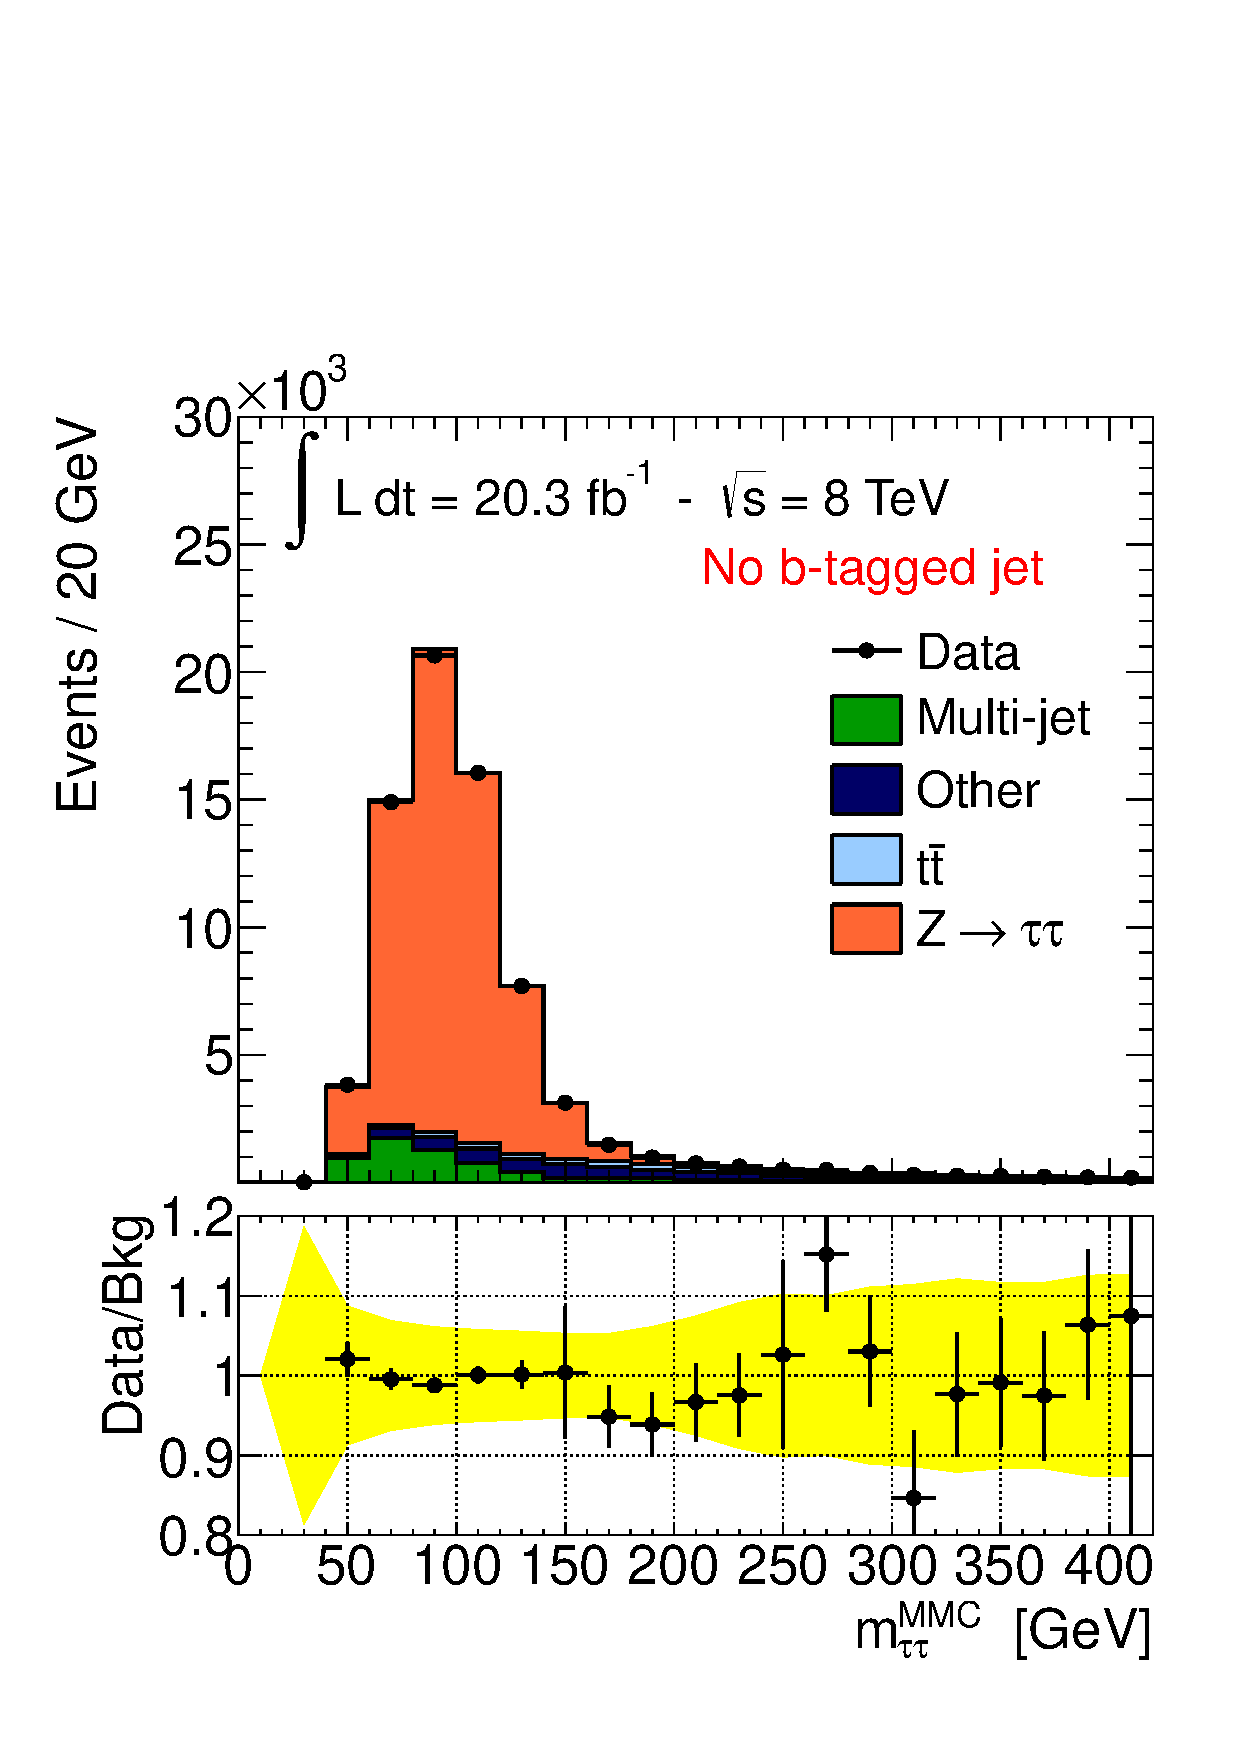
\includegraphics[width=0.47\textwidth]{figure/final_plots/std_presel_NoBtag_mmc_mass.pdf}
     }	
%     \subfigure[]{		
%            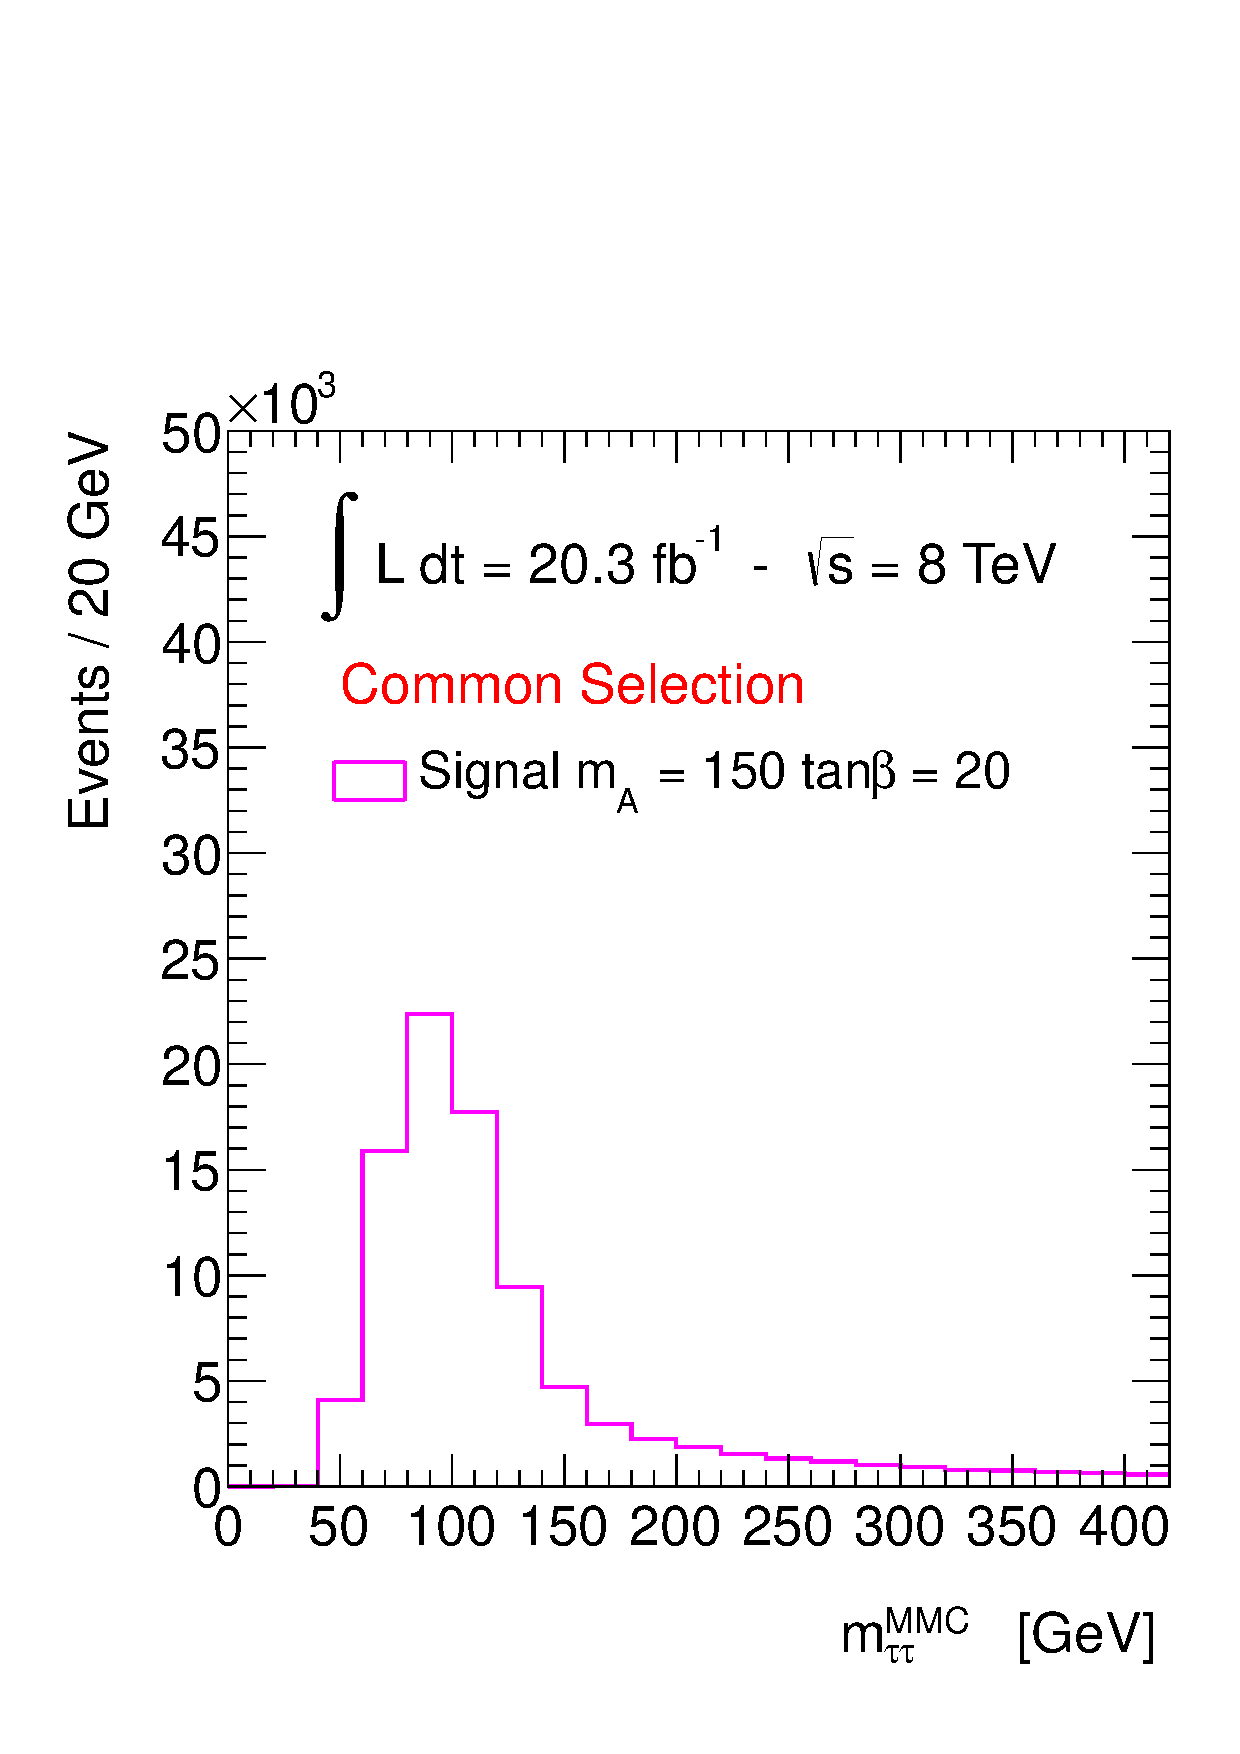
\includegraphics[width=0.47\textwidth]{figure/final_plots/signal_presel.pdf}
%     }	

    \end{center}
     	

    \caption{Observed and expected distribution of the 	invariant di-$\tau$ mass estimate \mmc at
	 different stage of the analysis: (a) after the common selection,
	(b) after requiring exactly one b-tagged jet and (c) for the b-vetoed sample.	The predictions 
	of the  background model is compared to  the data (as in Figure~\ref{fig:selections}).}
   \label{fig:mass}
\end{figure}


The accuracy of the  invariant mass obtained with the \mmc method depends strongly on the 
resolution of the missing transverse energy measurement.
To improve the $\met$ resolution, a scan of a six-dimensional parameter space is performed 
in a similar manner as described above. For this purpose, the absolute value of $\vec{E}_T^{miss}$ is also considered unknown and a scan 
is performed over all possible values constrained by the measured $\met$ and its corresponding uncertainty.
%on it assigning values  according to its uncertainty. 
%The probability of each solution is calculated and the final missing transverse
%energy is given by the weighted mean of the scanned points. 
%
%The final procedure consist in obtaining first an estimate for $\met$ by means of a six dimensional scan over the solution of equations~\ref{eq:MMC},
%successively a four dimensional scan is performed fixing $\met$ to the updated value and calculating the most likely invariant mass 
%of the di-$\tau$ system.

Figure~\ref{fig:mass} shows the  \mmc invariant mass distribution after the common selection and after the 
event categorization.

 
%Accurate invariant mass reconstruction of a di-tau system is a challenging task due to the escaping neutrinos.
%In this analysis, with four neutrinos in the final state, the number of unknown largely exceed the number of constraints,
%several approximation are possible to further constraint the neutrinos, for example assuming them collinear to the 
%other leptons from tau decay, however those approximation suffers of limitations. 

%In this analysis we use the so called missing mass calculator (MMC)~\cite{MMC}
%technique for the calculation of the di-tau system invariant mass. This technique employs additional 
%information from the well known tau decay to constraint the system, this is achieved by minimising a likelihood function 
%defined in the kinematically allowed phase space region, the result is a more precise measurement of the di-tau 
%system invariant mass and a considerable improvement in resolution. The invariant mass distribution 
%calculated with the MMC technique is referred in the following as $\mmc$ and is used as discriminating 
%variable in the limits setting.

